%%%%%%%%%%%%%%%%%%%%%%%%%%%%%%%%%%%%%%%%%%  不使用 authblk 包制作标题  %%%%%%%%%%%%%%%%%%%%%%%%%%%%%%%%%%%%%%%%%%%%%%
%-------------------------------PPT Title-------------------------------------
\title{22-选讲专题:~高通量计算材料流程与数据库}
%-----------------------------------------------------------------------------
%----------------------------Author & Date------------------------------------

%\author[\textrm{Jun\_Jiang}]{姜\;\;骏\inst{}} %[]{} (optional, use only with lots of authors)
%% - Give the names in the same order as the appear in the paper.
%% - Use the \inst{?} command only if the authors have different
%%   affiliation.
%\institute[BCC]{\inst{}%
\institute[Gain~Strong]{\inst{}%
%\vskip -20pt 北京市计算中心}
\vskip -20pt {\large 格致斯创~科技}}
\date[\today] % (optional, should be abbreviation of conference name)
{%	{\fontsize{6.2pt}{4.2pt}\selectfont{\textcolor{blue}{E-mail:~}\url{jiangjun@bcc.ac.cn}}}
\vskip 45 pt {\fontsize{8.2pt}{6.2pt}\selectfont{%清华大学\;\;物理系% 报告地点
	\vskip 5 pt \textrm{2023.04.22}}}
}

%% - Either use conference name or its abbreviation
%% - Not really information to the audience, more for people (including
%%   yourself) who are reading the slides onlin%%   yourself) who are reading the slides onlin%%   yourself) who are reading the slides onlineee
%%%%%%%%%%%%%%%%%%%%%%%%%%%%%%%%%%%%%%%%%%%%%%%%%%%%%%%%%%%%%%%%%%%%%%%%%%%%%%%%%%%%%%%%%%%%%%%%%%%%%%%%%%%%%%%%%%%%%

\subject{}
% This is only inserted into the PDF information catalog. Can be left
% out.
%\maketitle
\frame
{
%	\frametitle{\fontsize{9.5pt}{5.2pt}\selectfont{\textcolor{orange}{“高通量并发式材料计算算法与软件”年度检查}}}
\titlepage
}
%-----------------------------------------------------------------------------

%------------------------------------------------------------------------------列出全文 outline ---------------------------------------------------------------------------------
%\section*{}
%\frame[allowframebreaks]
%{
%  \frametitle{Outline}
%%  \frametitle{\textcolor{mycolor}{\secname}}
%  \tableofcontents%[current,currentsection,currentsubsection]
%}
%%在每个section之前列出全部Outline
%%类似的在每个subsection之前列出全部Outline是\AtBeginSubsection[]
%\AtBeginSection[]
%{
%  \frame<handout:0>%[allowframebreaks]
%  {
%    \frametitle{Outline}
%%全部Outline中,本部分加亮
%    \tableofcontents[current,currentsection]
%  }
%}

%-----------------------------------------------PPT main Body------------------------------------------------------------------------------------
\small
%\section{\rm{VASP~}软件中\rm{PAW~}计算的实现}
%\frame
%
%	\frametitle{\textrm{VASP}计算的特色}
%	相比于与普通的第一原理计算软件,\textrm{VASP}很好地平衡了计算效率和精度的问题,总的来说,\textrm{VASP}主要通过这几个特色保证了计算的高效能
%	\begin{itemize}
%	     \item 迭代与优化算法的多样性\\
%		     本质上电荷密度迭代 \textrm{\&\&} 体系总能量优化是相同的优化问题,采用了类似的算法\upcite{CMS6-15_1996,PRB54-11169_1996}:\\
%			\textcolor{blue}{\textrm{Pseudo-Newton、Conjugate-Gradient、Broyden~mix、damping-factor、RMM-DIIS}}
%	     \item 尽可能采用局域基(原子轨道基)函数:~\\
%		     \textcolor{blue}{\textrm{LREAL}}=\textcolor{red}{\textrm{.TRUE.}}\\
%			优化的投影函数也尽可能在实空间表示
%	     \item \textrm{PAW}原子数据集:\textcolor{blue}{优异的赝势}\upcite{PRB59-1758_1999}
%	\end{itemize}
%}
\section{高通量计算材料自动流程}
\frame
{
	\frametitle{高通量计算流程}
高通量\footnote{\fontsize{5.5pt}{4.2pt}\selectfont{高通量的概念最初出现在实验领域,早期的材料研究、制药研究主要通过大量备选材料试错,最终才得到合适的材料或药物重要功能成分,这就是一种高通量筛选。文献中常会提到“高通量”和“组合方法”(\textrm{Combinational approach}),但很少区分两者的区别:~“高通量”指用户产生或处理的数据量极大,没有计算机自动处理无法完成;~而“组合方法”是针对影响研究对象的各种可能自由度的分门别类研究。换言之,高通量考虑的是利用计算机“一视同仁”地自动化式处理海量数据,而组合方法更强调对特定影响因素的筛查和组合研究}}计算流程主要任务包括三方面:
\begin{itemize}
	\item \textcolor{blue}{增加材料模拟数据}:~主要包括\textrm{DFT}、\textrm{MD}计算的材料数据
	\item \textcolor{blue}{存储材料物性数据}:~系统存储材料数据,用以构建材料数据库
		\vskip 2pt
		{\fontsize{6.5pt}{4.2pt}\selectfont{材料数据库包括通用材料数据库或特定目标的材料数据库}}
\item \textcolor{blue}{检索材料数据}:~对存储的材料数据实施检索和分析,服务材料性能提升需求
\end{itemize}
高通量计算流程的主要目标之一就是构建材料数据库
\vskip 2pt
{\fontsize{7.5pt}{4.2pt}\selectfont{\textcolor{cyan}{高通量计算流程与数据密不可分:~著名的高通量计算流程都有相应的数据库}
\begin{itemize}
	\item \textrm{AFLOW}的数据库为\textrm{AFLOWLIB}
	\item \textrm{MP}的数据库为同名的\textrm{Materials Project}
	\item \textrm{ASE}的数据库为\textrm{CMR~(The Computational Materials Repository)}
\end{itemize}
%,,。中科院物理所也拥有一个通用的材料科学数据库\textrm{Atomly}
}}
}

\frame
{
	\frametitle{国外已有的计算平台}
\begin{figure}[h!]
\centering
\vspace{-15.5pt}
\subfigure[\fontsize{6.5pt}{6.2pt}\selectfont{\textrm{Auto-FLOW (AFLOW)}\upcite{CMS58-227_2012}}]{
\label{AFLOW_data_flow}
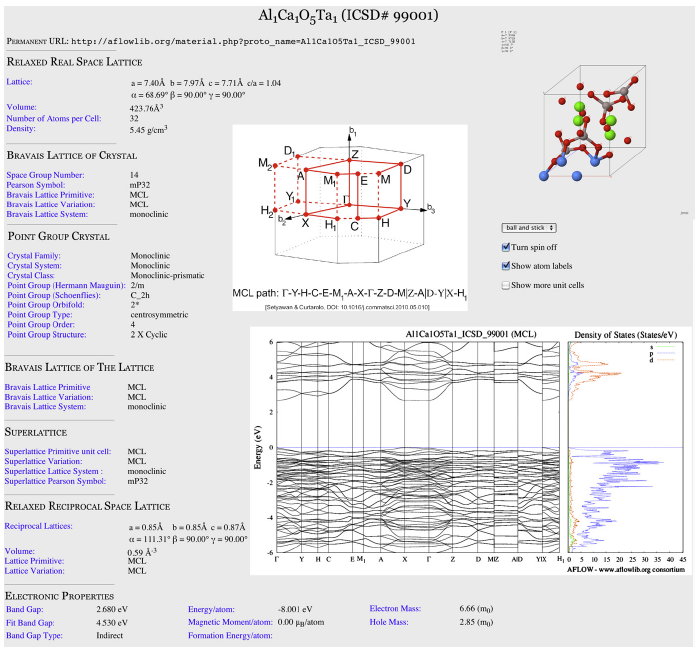
\includegraphics[height=1.2in,width=1.6in,viewport=0 0 720 660,clip]{Figures/AFLOW_database.png}}
\subfigure[\fontsize{6.5pt}{6.2pt}\selectfont{\textrm{Material Project (MP)}\upcite{CMS97-209_2015}}]{
\label{MP_commp_infrastructure}
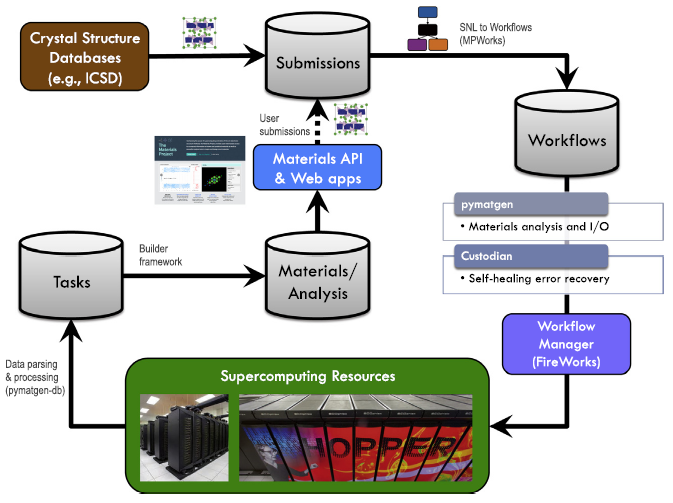
\includegraphics[height=1.2in,width=1.7in,viewport=0 0 670 530,clip]{Figures/MP_comp_infrastructure.png}}
\subfigure[\fontsize{3.5pt}{3.2pt}\selectfont{\textrm{Quantum Materials Informatics Project (QMIP)}\upcite{url_QMIP}}]{
\label{QMIP_Shame}
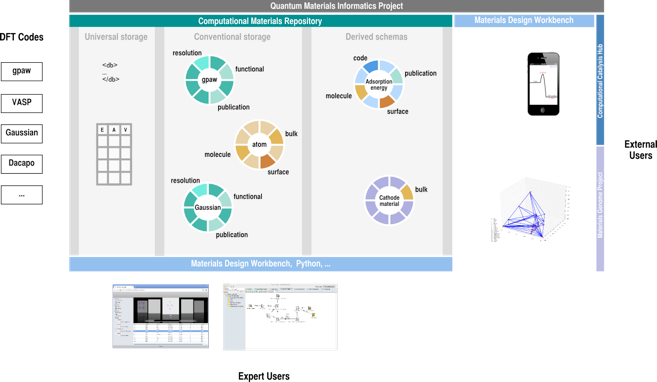
\includegraphics[height=1.2in,width=1.7in,viewport=0 0 670 420,clip]{Figures/QMIP_shame.png}}
\subfigure[\fontsize{6.5pt}{5.2pt}\selectfont{\textrm{Clean Energy Project (CEP)}\upcite{JPCL2-2241_2011}}]{
\label{CEP_structure_flow}
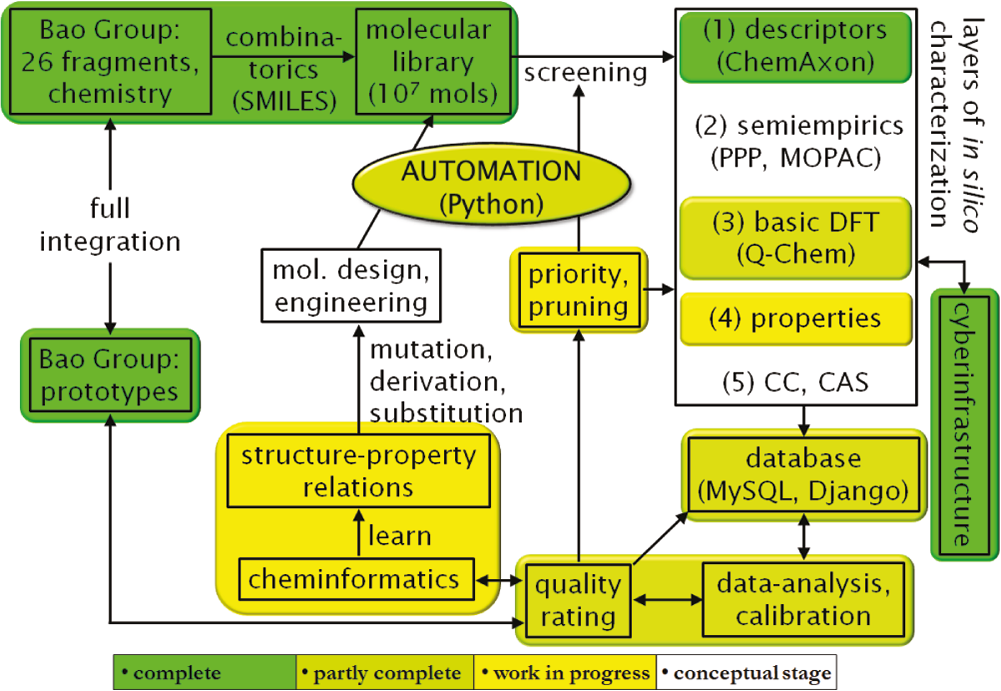
\includegraphics[height=1.2in,width=1.6in,viewport=0 0 1020 730,clip]{Figures/CEP_structure_flow.png}}
%\caption{}%
\label{Auto_Flow_Platform-1}
\end{figure}
}

\frame
{
	\frametitle{国内已有的计算平台:~\textrm{MatCloud}}
\begin{figure}[h!]:
\centering
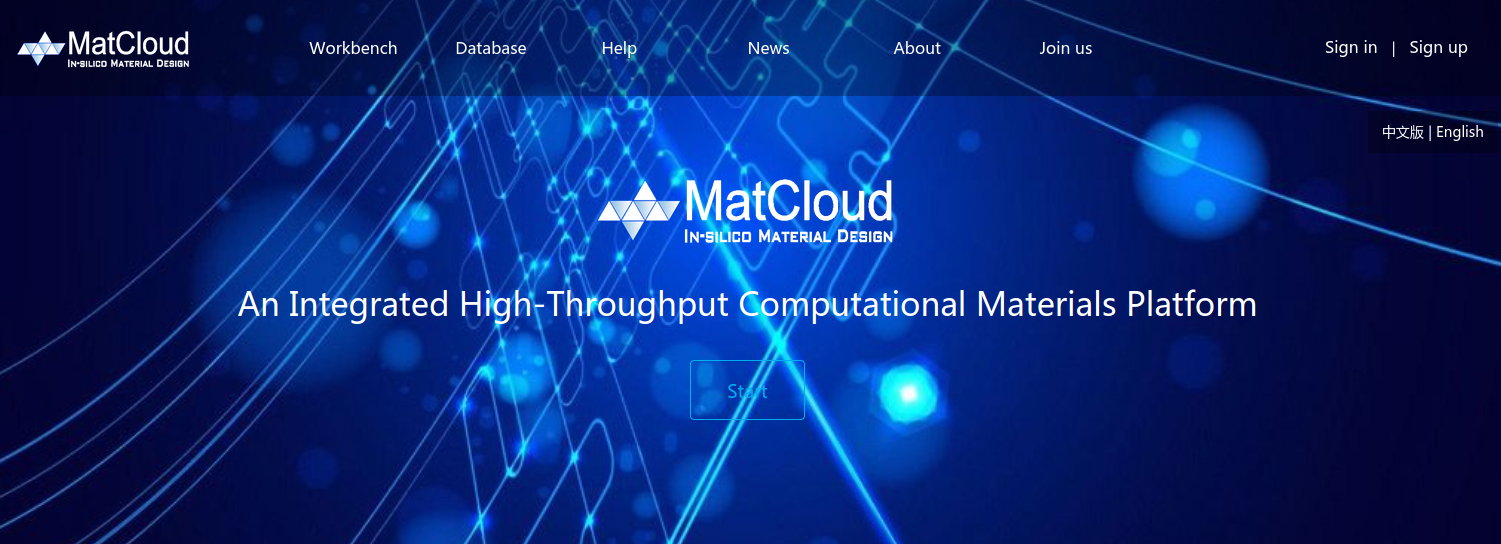
\includegraphics[height=1.57in,width=4.95in,viewport=0 0 1800 550,clip]{Figures/Matcloud-login.png}
\caption{\fontsize{7.2pt}{4.2pt}\selectfont{中科院计算机网络信息中心~杨小渝团队开发}\upcite{CMS146-319_2018,url_Matcloud}}%
\label{Auto_Flow_Platform-2}
\end{figure}
}

\frame
{
	\frametitle{高通量计算自动流程} 
当前高通量计算的自动处理流程集中在材料模拟的计算数据收集和实现计算结果自动入库为主
\vskip 2pt
{\fontsize{7.5pt}{4.2pt}\selectfont{材料第一原理计算的软件有很多,输出文件的格式千差万别,通过第一原理计算构建相对完善的材料数据库需要耗费相当的计算资源和人力}}
\vskip 5pt
自动流程面向的对象是数据,要实现材料计算过程的自动处理,首先需要解决的是数据格式的规范化
\begin{itemize}
	\item \textcolor{magenta}{数据规范化类型}:~面向各类软件输出数据的自动化提取与传输
\vskip 2pt
{\fontsize{6.5pt}{4.2pt}\selectfont{根据软件的计算特点,组织多种软件实现材料物性计算:~\textcolor{blue}{灵活性较好,但一般只支持相对简单的计算流程}}}
\item \textcolor{magenta}{流程规范化类型}:~面向材料计算软件的标准化流程,通过数据库支持 
\vskip 2pt
{\fontsize{6.5pt}{4.2pt}\selectfont{利用数据库技术将自动流程组织得更复杂多样,并作为数据库条目存储下来:~\textcolor{blue}{稳定性较好,但计算的材料物性受软件能力的限制较多}}}
\end{itemize}
\textcolor{purple}{主要的自动流程采用\textrm{Python}语言实现}:~跨平台、模块化组织灵活
}

\frame
{
	\frametitle{计算平台的功能和总体架构}
\begin{figure}[h!]
\centering
\vspace*{-0.35in}
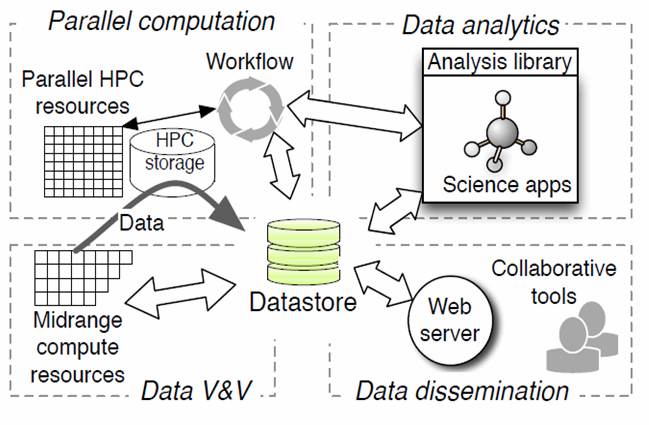
\includegraphics[height=2.6in,width=4.05in,viewport=0 0 670 460,clip]{Figures/Parallel_computation.png}
%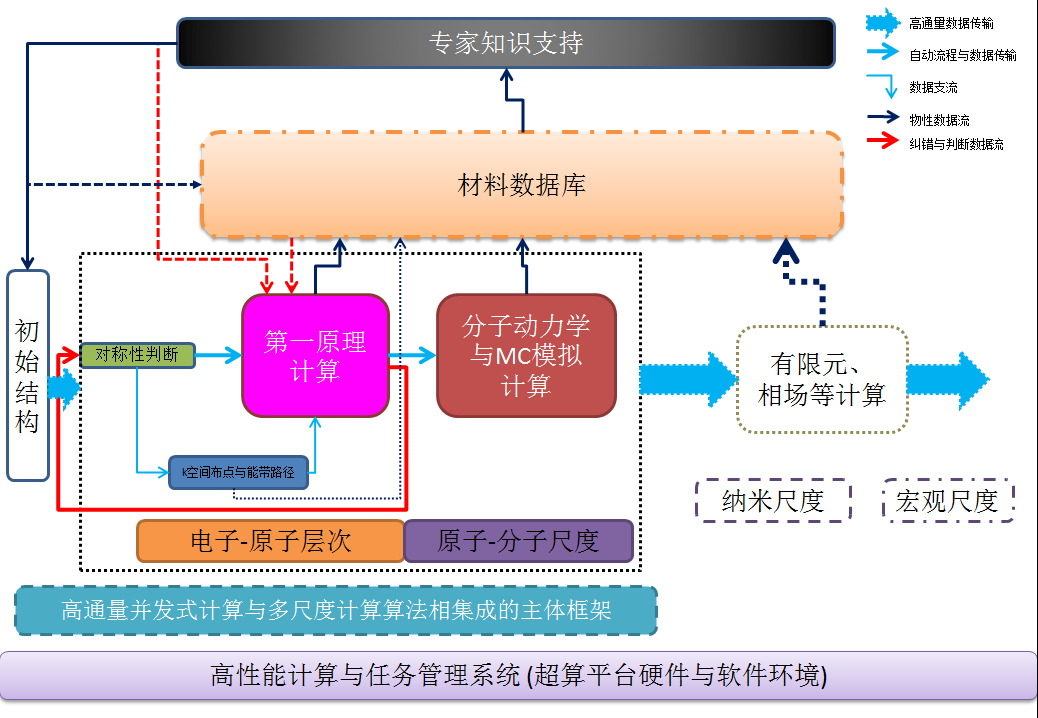
\includegraphics[height=1.6in,width=2.4in,viewport=0 0 1038 730,clip]{Figures/Auto_Flow.png}
\caption{\fontsize{7.2pt}{4.2pt}\selectfont{\textrm{The schematic framework and platform of all those project.}}}%
\label{Auto_Flow}
\end{figure} 
}

\frame
{
	\frametitle{材料计算软件发展现状}
\begin{figure}[h!]
\vspace*{-0.16in}
\centering
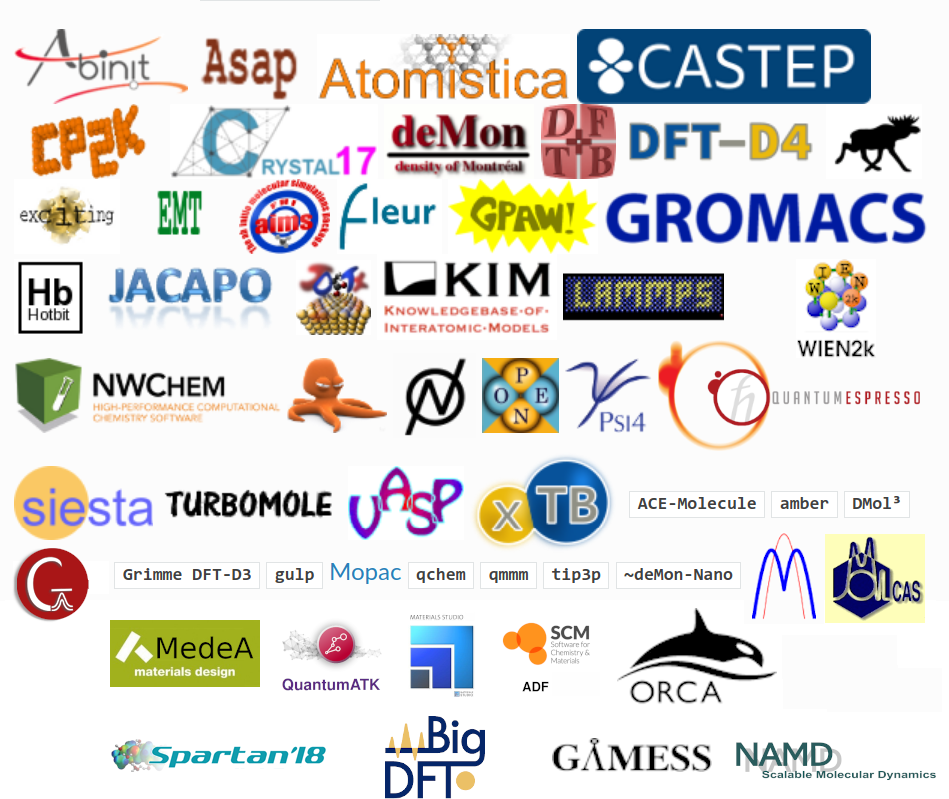
\includegraphics[width=3.30in]{Figures/Softwares_logo.png}
%\caption{\tiny \textrm{Pseudopotential for metallic sodium, based on the empty core model and screened by the Thomas-Fermi dielectric function.}}%(与文献\cite{EPJB33-47_2003}图1对比)
\label{Softwares}
\end{figure}
}

\frame
{
	\frametitle{国产第一原理计算软件现状}
\begin{figure}[h!]
\vspace*{-0.19in}
\centering
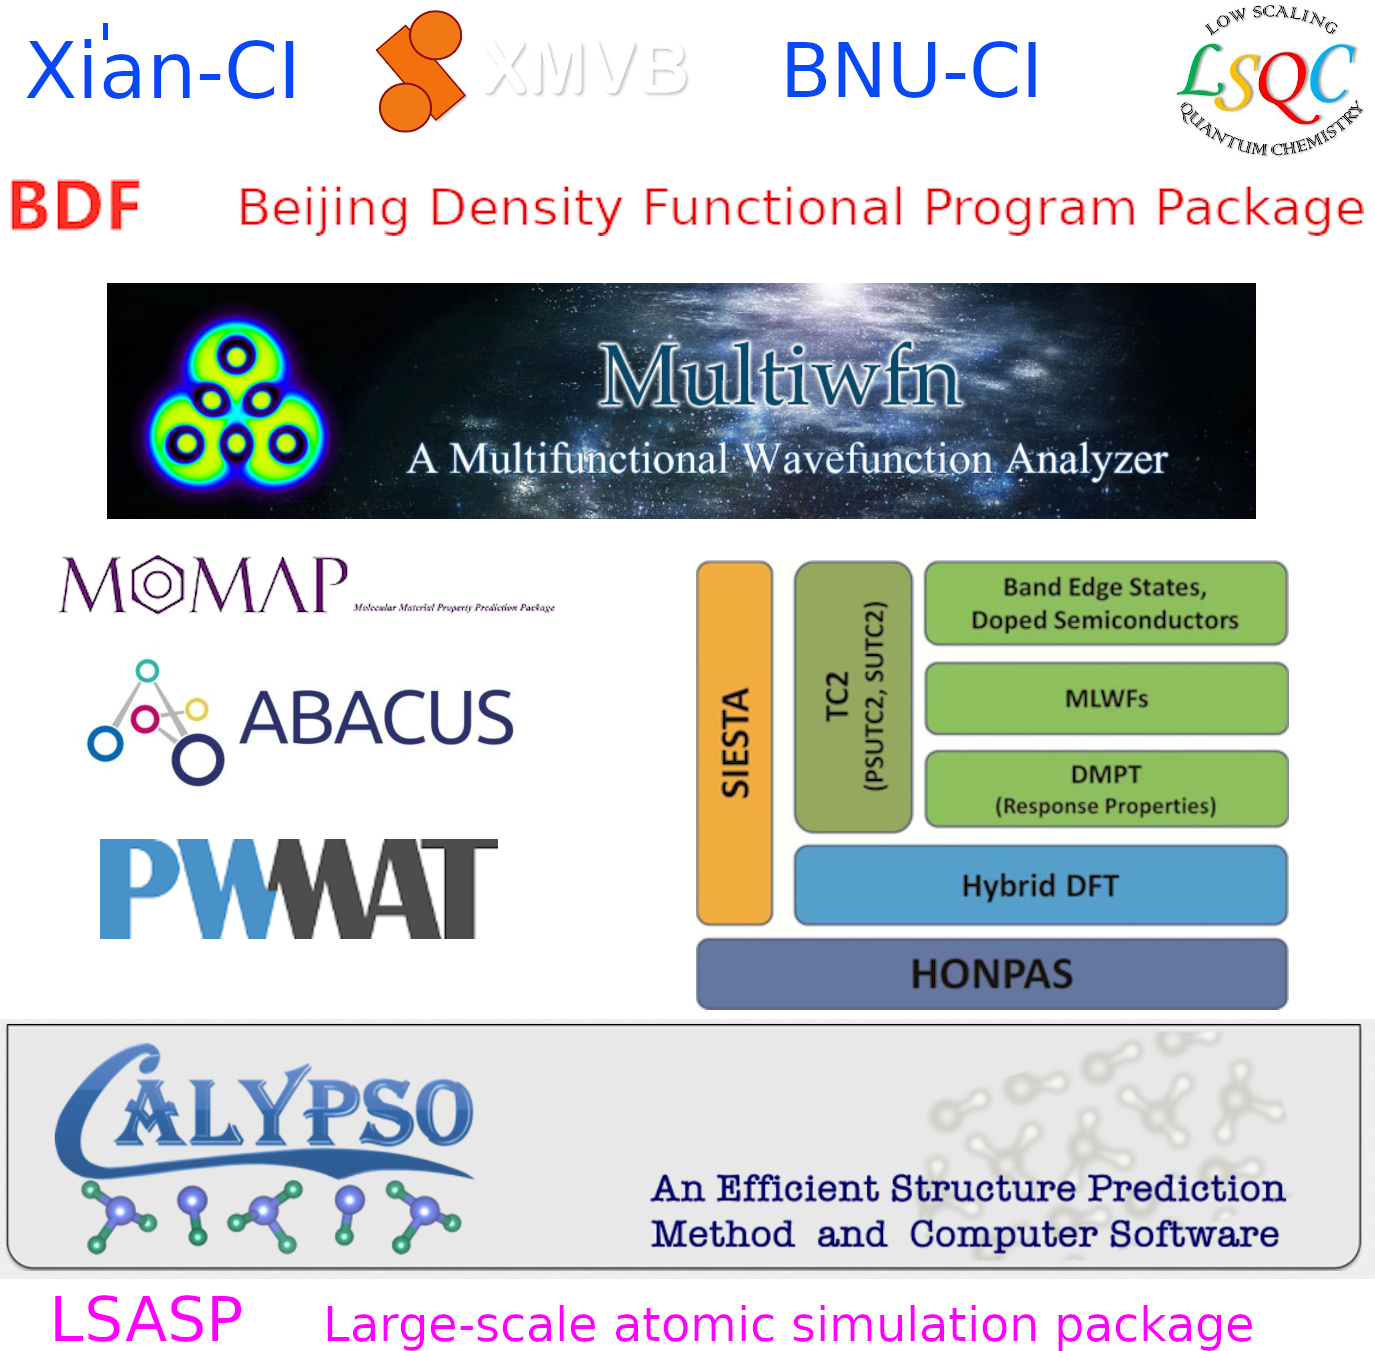
\includegraphics[width=2.83in]{Figures/Softwares_China-logo.png}
%\caption{\tiny \textrm{Pseudopotential for metallic sodium, based on the empty core model and screened by the Thomas-Fermi dielectric function.}}%(与文献\cite{EPJB33-47_2003}图1对比)
\label{Software-China}
\end{figure}
	\fontsize{6.2pt}{5.2pt}\selectfont{\textcolor{red}{中国学科发展战略\,$\cdot$\,理论与计算化学,~~国家自然科学基金委员会,~中国科学院,~~北京:~科学出版社,~~2016}}
}

\frame
{
	\frametitle{\textrm{ASE}自动流程的设计与管理}
数据规范化型的自动处理以\textrm{ASE}为典型代表,通过各类\textrm{Python}模块,支持多种\textrm{DFT-MD}软件%。根据图\ref{Auto_Flow_Platform-5}可知,\textrm{ASE}的核心模块主要包括\textrm{Atoms}(原子、分子建模)、\textrm{Calculator}(各类计算软件运行支持与控制)和物性计算、功能分析和结果可视化模块。
\vskip 3pt
		\textcolor{purple}{\textrm{ASE}特色}:~模块加载式计算流程控制,符合复杂多尺度计算场景
		\begin{itemize}
			\item \textcolor{magenta}{灵活的建模功能}
				\begin{enumerate}
    \setlength{\itemsep}{7pt}
					\item 简单组织:~原子直接构成分子
					\item 理想周期体系(包括一维、二维、三维)
					\item 表面和表面吸附,可指定吸附位
				\end{enumerate}
			\item \textcolor{magenta}{丰富的软件接口}\\
				提供了包括绝大部分第一原理和分子动力学计算软件接口,方便组合实现多尺度计算
			\item \textcolor{magenta}{不依赖软件的优化与动力学模拟}\\
				适合复杂材料物性模拟的优化和多种动力学过程模拟
			\item \textcolor{magenta}{多样化的数据库类型}
		\end{itemize} 
}

\frame
{
\frametitle{\textrm{ASE}的结构生成模块}
\begin{minipage}[b]{0.48\textwidth}
	{\fontsize{7.8pt}{5.2pt}\selectfont{
	材料结构生成模块主要功能:}}
	{\fontsize{6.2pt}{5.2pt}\selectfont{
\begin{itemize}
    \setlength{\itemsep}{4pt}
	\item 生成各种计算软件所需的结构模型
		\vskip 1pt
		包括原子、分子、晶体、表面和界面等
	\item 读入各种格式的结构模型文件
		\vskip 1pt
		包括\texttt{xyz}、\textrm{POSCAR}、\texttt{cif}等\textrm{65}种格式
	\item 各类结构模型统一以\texttt{traj}或\texttt{json}格式写入数据库
		\vskip 1pt
		实现计算模型数据的标准化
\end{itemize}}}
\begin{figure}[h!]
\centering
\vspace*{-0.15in}
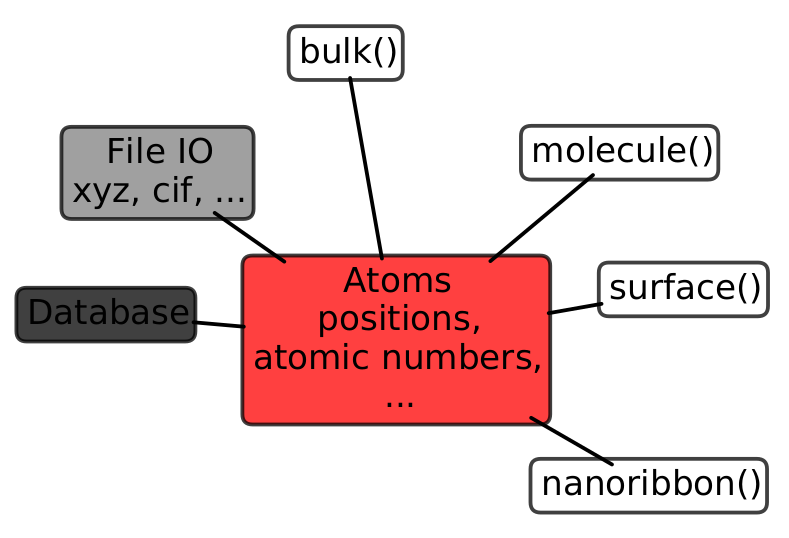
\includegraphics[height=1.3in,width=1.9in,viewport=0 0 820 530,clip]{Figures/ASE_atoms_module.png}
%\caption{\fontsize{7.2pt}{4.2pt}\selectfont{\textrm{The integrated calculator in ASE (Atomic Simulation Environment).}}}%
\label{Logo_atoms-module}
\end{figure} 
\hfill
\end{minipage}
\begin{minipage}[b]{0.50\textwidth}
\begin{figure}[h!]
\centering
\vspace*{-0.15in}
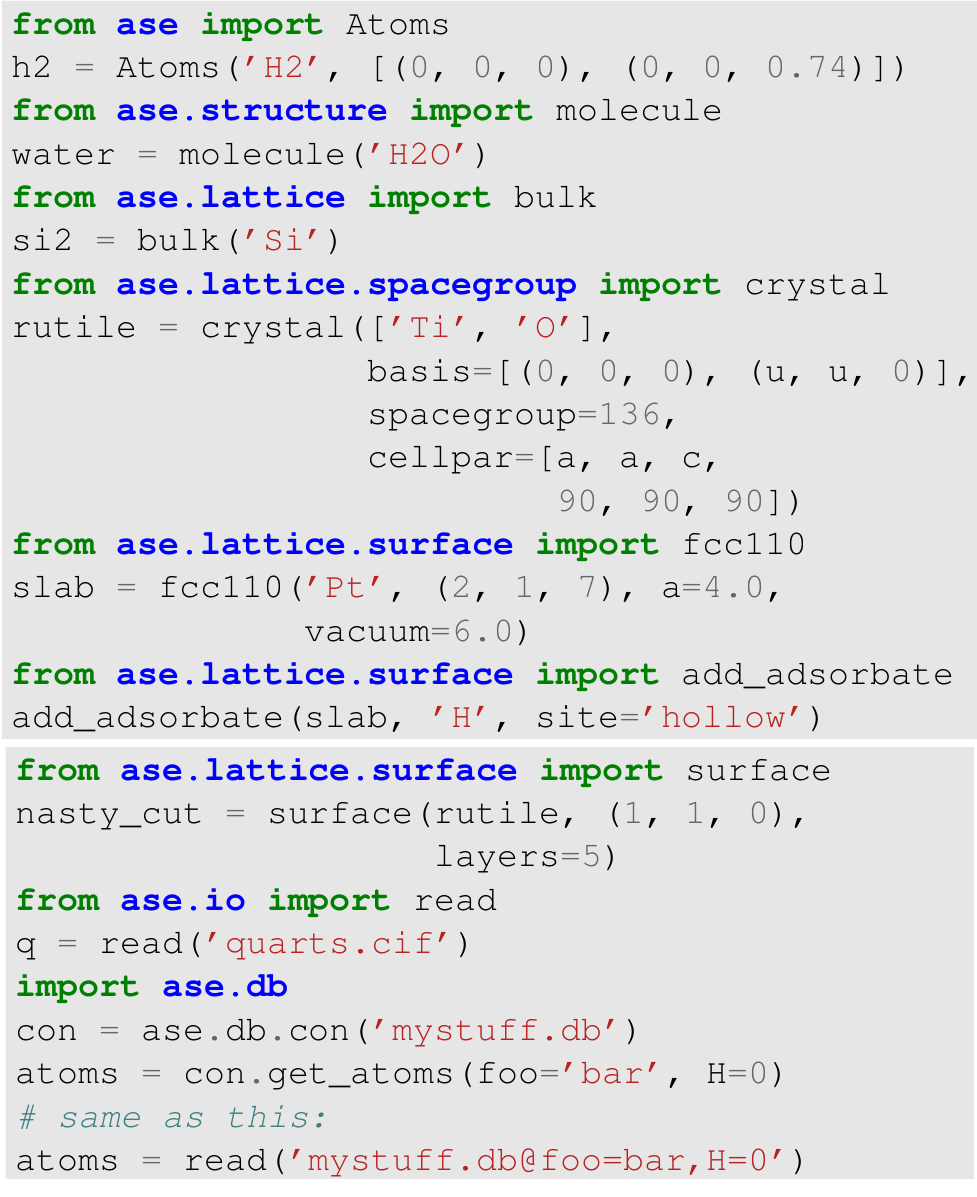
\includegraphics[height=2.9in,width=2.2in,viewport=0 0 970 1200,clip]{Figures/ASE_atoms_module-examples.png}
%\caption{\fontsize{7.2pt}{4.2pt}\selectfont{\textrm{The integrated calculator in ASE (Atomic Simulation Environment).}}}%
\label{Logo_atoms-module}
\end{figure} 
\end{minipage}
}

\frame
{
\frametitle{\textrm{ASE}特色:~软件接口丰富}
\textrm{Calculator}模块支持的可选软件
\begin{figure}[h!]
\centering
\vspace*{-0.05in}
%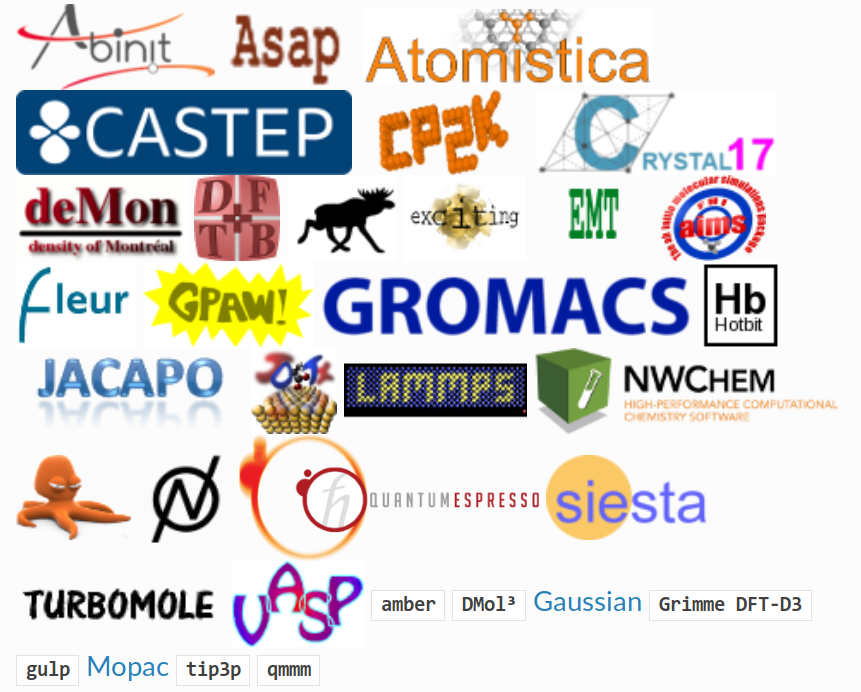
\includegraphics[height=1.0in,width=1.4in,viewport=0 0 638 530,clip]{Figures/ASE_calculator.png}
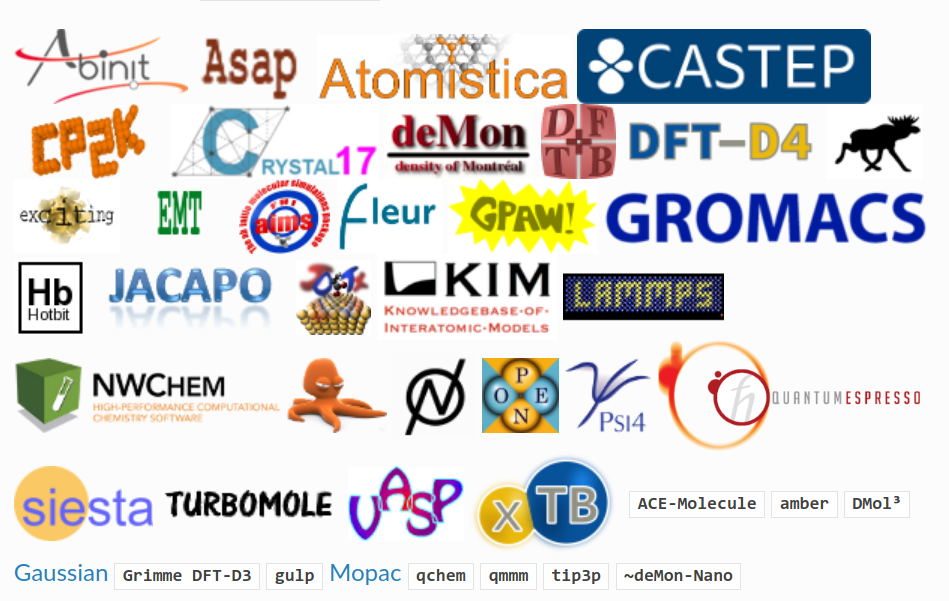
\includegraphics[height=2.4in,width=3.8in,viewport=0 0 940 600,clip]{Figures/ASE_calculator-new.png}
\caption{\fontsize{6.2pt}{4.2pt}\selectfont{\textrm{The integrated calculator in ASE.}}}%
\label{ASE_Calculator}
\end{figure} 
}

\frame
{
	\frametitle{\textrm{ASE}的模块:~\textrm{Calculator}和\textrm{checkpointing}}
\textrm{Calculator}:~支持各类计算软件的主要模块
	{\fontsize{8.0pt}{5.2pt}\selectfont{
\begin{itemize}
	\item 模块封装了\textrm{DFT-MD}计算软件,支持物性计算、功能分析
	\item 模块集成了全局结构搜索算法(\textrm{Base-hopping}和\textrm{minima-hopping}算法)、反应动力学模拟\textrm{NEB}算法和势能面鞍点搜索算法、\textrm{MD}模拟算法、几何结构优化算法和分子振动与声子振动分析算法
	\item 模块支持材料物性自动化计算,数据以标准化形式存入数据库
\end{itemize}
		模块启动计算依次执行以下步骤:
\begin{enumerate}
	\item 生成计算软件所需的输入(控制)文件
	\item 启动软件,以子进程方式开始计算过程
	\item 进程守护直至计算子进程结束
	\item 根据要求解析计算软件生成文件,并可将计算结果以\texttt{json}格式写入数据库
\end{enumerate}}}
{\fontsize{7.5pt}{5.2pt}\selectfont{
	\begin{itemize}
		\item \textcolor{red}{优点}:~\textrm{Python}模块与计算软件的交互简单
		\item \textcolor{red}{缺点}:~\textrm{Python}执行过程中会面向较多的\textrm{I/O}处理,运行效率不高
	\end{itemize} }}
\textrm{checkpointing}:~协助用户排查、定位错误和重启计算的模块
\vskip 2pt
{\fontsize{7.5pt}{5.2pt}\selectfont{增加\textrm{ASE}对计算流程的控制能力}}
}

\frame
{
\frametitle{\textrm{ASE}特色:~数据库的良好兼容性}
\begin{minipage}[b]{0.38\textwidth}
{\fontsize{7.5pt}{5.2pt}\selectfont{
\textrm{ASE}的材料数据库\textrm{CMR}采用关系型数据库管理系统\textrm{MySQL}
\vskip 1pt
{\fontsize{6.0pt}{5.2pt}\selectfont{将规范化的数据转成数据库文件(称为\textit{cmr}-文件),并要求数据库中的文件名尽可能与原文件保持一致}}
\begin{itemize}
	\item 用户不进入数据库即可对数据进行检验
	\item 存储数据有更大的兼容性
	\item 
	\item
\end{itemize}}}
\end{minipage}
\hfill
\begin{minipage}[b]{0.60\textwidth}
\begin{figure}[h!]
\centering
\vspace*{-0.10in}
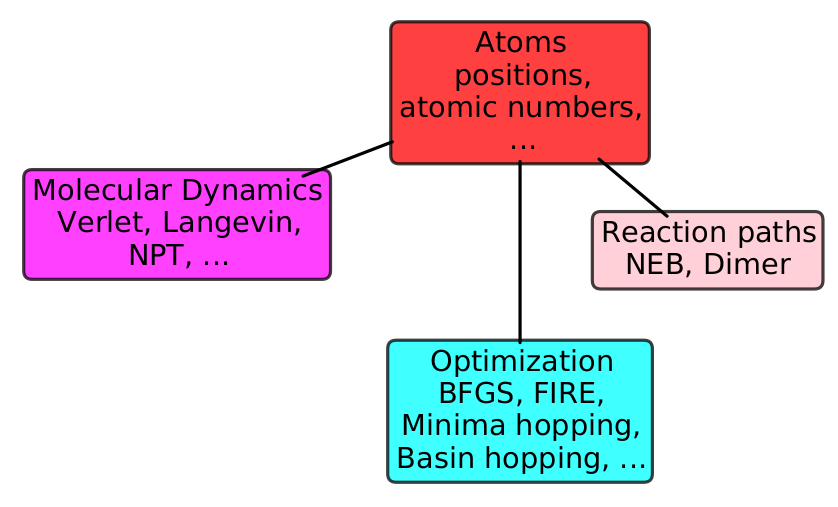
\includegraphics[height=1.3in,width=2.5in,viewport=0 0 838 500,clip]{Figures/ASE_opt_modules.png}
\vskip 1pt
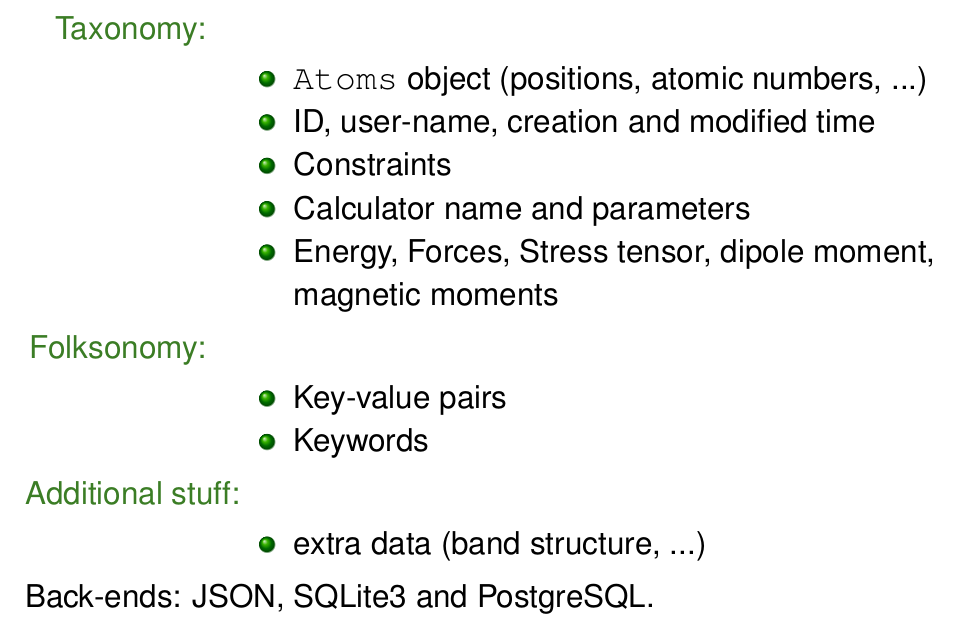
\includegraphics[height=1.7in,width=2.5in,viewport=0 0 938 630,clip]{Figures/ASE_database.png}
\label{ASE_opt-database}
\end{figure} 
\end{minipage}
}

\frame
{
	\frametitle{\textrm{MP}自动流程的架构}
流程标准化型的自动处理以\textrm{MP}的流程控制\textrm{FireWorks}为代表
	\begin{itemize}
		\item \textcolor{red}{设计目标}:~围绕\textrm{VASP~}作业高通量并发提交与过程监控
		\item \textcolor{red}{设计方案}:~开发针对不同计算场景的功能模块
			\begin{enumerate}
    \setlength{\itemsep}{7pt}
				\item \textcolor{blue}{\textbf{Pymatgen}}\\
					\textcolor{magenta}{前处理}:~计算模型的分析与预处理\\
					\textcolor{magenta}{后处理}:~计算结果的可视化
				\item \textcolor{blue}{\textbf{FireWorks}}\\
					\textcolor{magenta}{数据库支持的计算流程设计与管理}:~复杂的工作流可以数据形式保存到\textrm{MongoDB}数据库中,用\textrm{FireWorks}设计的工作流具有较高的稳定性
				\item \textcolor{blue}{\textbf{Custodian}}\\
\textcolor{magenta}{计算流程容错与应对}:~提供计算过程错误判断接口,由用户提供解决策略和针对性设计
			\end{enumerate}
	\end{itemize}
		%\item 计算过程的控制方式
}

\frame
{
	\frametitle{\textrm{Pymatgen}的模块结构}
\begin{figure}[h!]
\centering
\vspace*{-0.1in}
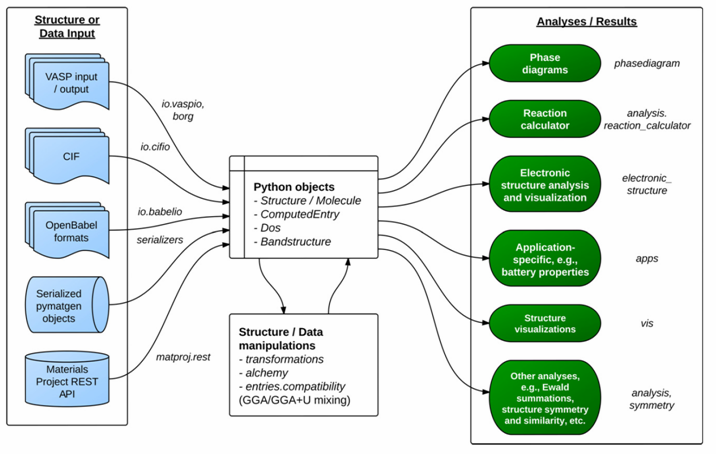
\includegraphics[height=2.3in]{Figures/MP_library.png}
\caption{\fontsize{7.2pt}{4.2pt}\selectfont{\textrm{Overview of a typical workflow for pymatgen.}}}%
\label{Pymatgen_Lib}
\end{figure} 
}

\frame
{
	\frametitle{\textrm{Pymatgen}可展示的材料物性}
\begin{figure}[h!]
\centering
\vspace*{-0.1in}
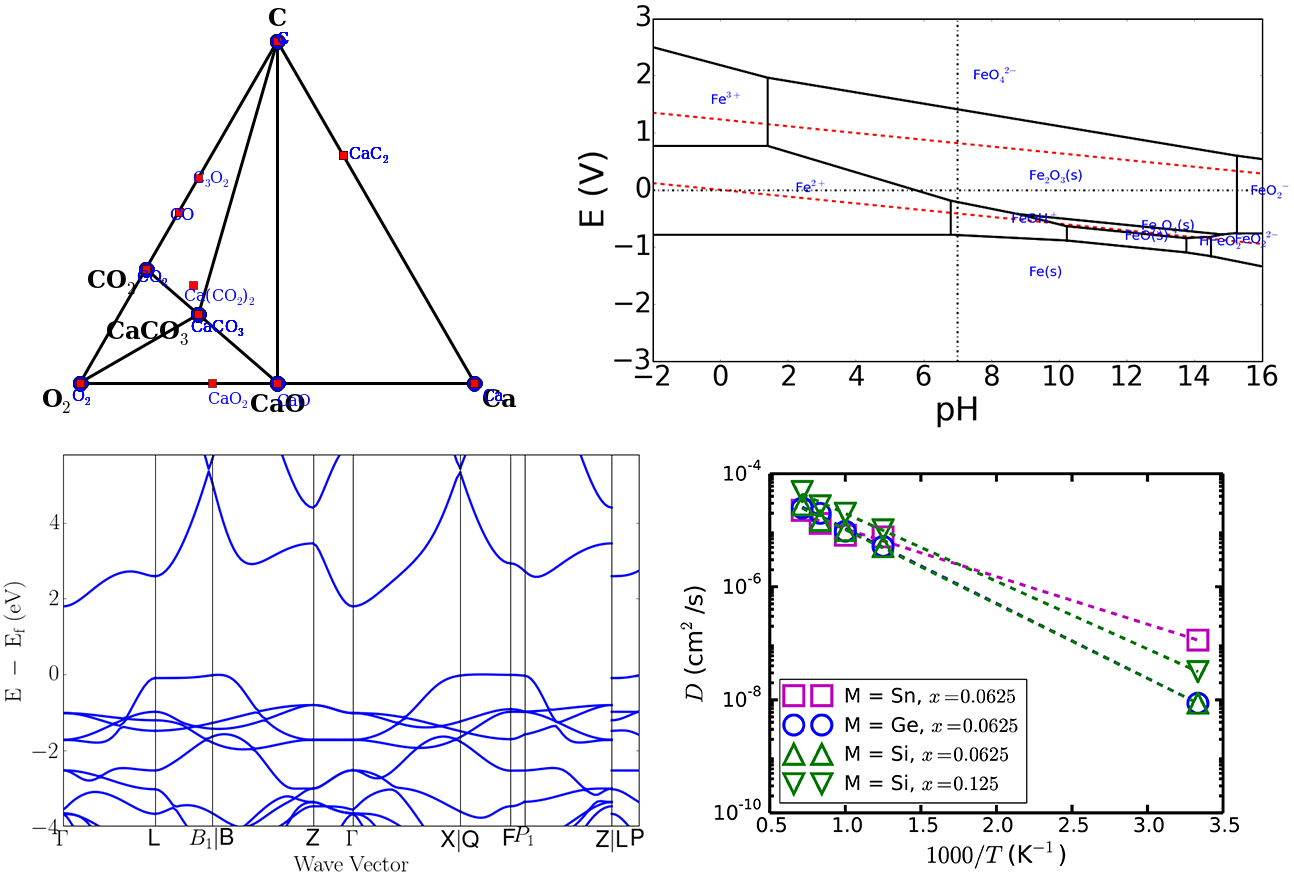
\includegraphics[height=2.3in]{Figures/MP_vision.png}
\caption{\fontsize{5.2pt}{4.2pt}\selectfont{\textrm{Top left: Phase; Top right: Pourbaix diagram from the Materials API. \\Bottom left: Calculated bandstructure plot using pymatgen’s parsing and plotting utilities. Bottom right: Arrhenius plot using pymatgen’s Diffusion~Analyzer.}}}%
\label{Pymatgen_vision}
\end{figure} 
}

\frame
{
	\frametitle{\textrm{FireWorks}的模块结构}
\textrm{FireWorks}是一款开源的通用工作流定义、管理和执行软件,支持\textrm{Python}运行
\vskip 3pt
\textrm{FireWorks}的自动流程采取中心化的“发布-执行”模式
\begin{itemize}
    \setlength{\itemsep}{7pt}
	\item 流程发布(称为\textrm{LachPad}):\\
		{\fontsize{7.2pt}{4.2pt}\selectfont{\textrm{LaunchPad}是工作流的主管者,主要负责自动流程的定义、分发、排队、增删和对工作流的反馈与响应}}
	\item 流程执行(称为\textrm{FireWorkers}):\\
		{\fontsize{7.2pt}{4.2pt}\selectfont{\textrm{FireWorkers}是工作流的执行者,包括一个或多个计算资源(个人计算机、小型工作站、超级计算机等)}}
\end{itemize}
\textrm{FireWorkers}从\textrm{LaunchPad}处获得计算任务,执行完毕后再将计算结果返回到\textrm{LaunchPad}
}

\frame
{
	\frametitle{\textrm{FireWorks}的模块结构}
\begin{figure}[h!]
\centering
\vspace*{-0.05in}
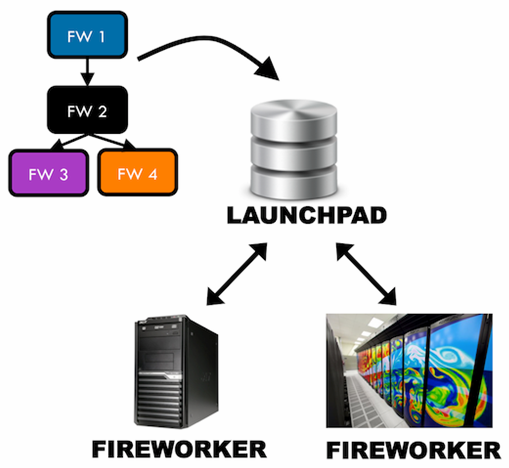
\includegraphics[height=1.5in]{Figures/MP_fireworks.png}
\hskip 1pt
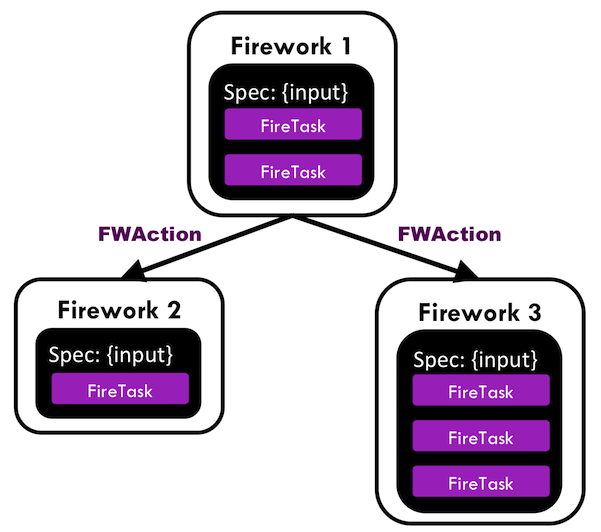
\includegraphics[height=1.5in]{Figures/MP_multiple_fw.png}
\caption{\fontsize{7.2pt}{4.2pt}\selectfont{\textrm{The basic infrastructure of FireWorks.}}}%
\label{FireWorks_FW}
\end{figure} 
\textrm{FireWorks}发布的工作流程由三层嵌套结构组成:
\fontsize{8.2pt}{6.2pt}\selectfont{
\begin{itemize}
	\item \textrm{Firetask}:~基本执行单元,是执行计算的最基本脚本命令或\textrm{Python}命令。
	\item \textrm{Firework}:~组织基本执行单元构成任务单元组,并指定各基本执行单元所需的参数。
	\item \textrm{Workflow}:~彼此相关联的任务单元组构成完整的工作流程:\\
		\textrm{FireWork}之间的数据传递、任务执行序列等由\textrm{FWAction}完成。
\end{itemize}}
}

\frame
{
	\frametitle{\textrm{FireWorks}的模块结构}
\fontsize{8.2pt}{6.2pt}\selectfont{
	\begin{itemize}
		\item \textrm{FireWorks}是以任务单元组为基本组成的来实现工作流程的,任务单元组之间依靠数据传递相关联,流程执行完毕也将返回数据,\textrm{FWAction}模块主要负责任务单元组之间的数据传递和任务分配。
		\item \textrm{FWAction}允许用户根据需要设计和更改流程参数、增添、删减和改变流程(子)单元组,这一模块大大增加了\textrm{FireWorks}工作流的灵活性。
	\end{itemize}}
\begin{figure}[h!]
\centering
\vspace*{-0.10in}
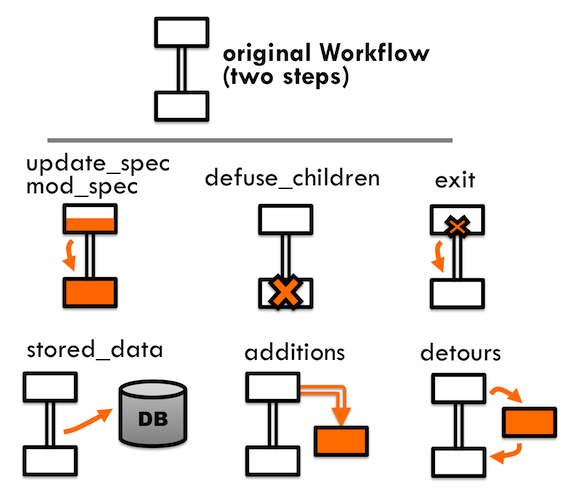
\includegraphics[height=1.9in]{Figures/MP_Fireworks_fwactions.png}
\caption{\fontsize{7.2pt}{4.2pt}\selectfont{\textrm{FireWorks}的单元组间数据传递与处理示意.}}%
\label{FireWorks_FWA}
\end{figure} 
}

\frame
{
	\frametitle{\textrm{FireWorks}的模块结构}
这种“发布-执行”结构使得计算任务与软件、硬件高度解耦,用户可根据需要随时向\textrm{LaunchPad}添加新的工作流,承担计算任务的\textrm{FireWorkers}彼此也可以是完全异构的,具有很好的机动性。
\vskip 0.25in
对于材料第一原理计算自动流程而言,一个\textrm{DFT}计算过程就是一个\textrm{Firework},可以分解为:
\begin{enumerate}
	\item 指定控制参数:~参数在数据库\texttt{Json}中存储,由\textrm{Spec}传入
	\item 计算控制文件生成:~每个\textrm{Firetask}生成一个控制文件
	\item \textrm{DFT}计算作业提交:~产生一个\textrm{Firetask}
\end{enumerate}
在此基础上,可以通过\textrm{FWAction}修改控制参数,将\textrm{DFT}计算单元组组织成完整的材料第一原理计算流程,并将最终结果直接导入材料计算数据库。
}

\frame
{
	\frametitle{\textrm{Custodian}的容错逻辑}
\begin{figure}[h!]
\centering
\vspace*{-0.1in}
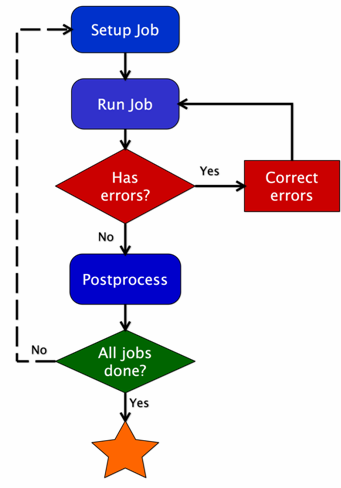
\includegraphics[height=2.7in]{Figures/MP_custodian.png}
\label{Custodian_over}
\caption{\fontsize{7.2pt}{4.2pt}\selectfont{\textrm{Overview of the Custodian workflow.}}}%
\end{figure} 
}

\frame
{
	\frametitle{\textrm{atomate}:~计算流程控制示范}
%		\textcolor{purple}{\textrm{Atomate}}:~:~适合一定复杂程度的\textrm{~VASP~}计算
\begin{figure}[h!]
\centering
\vspace*{-0.19in}
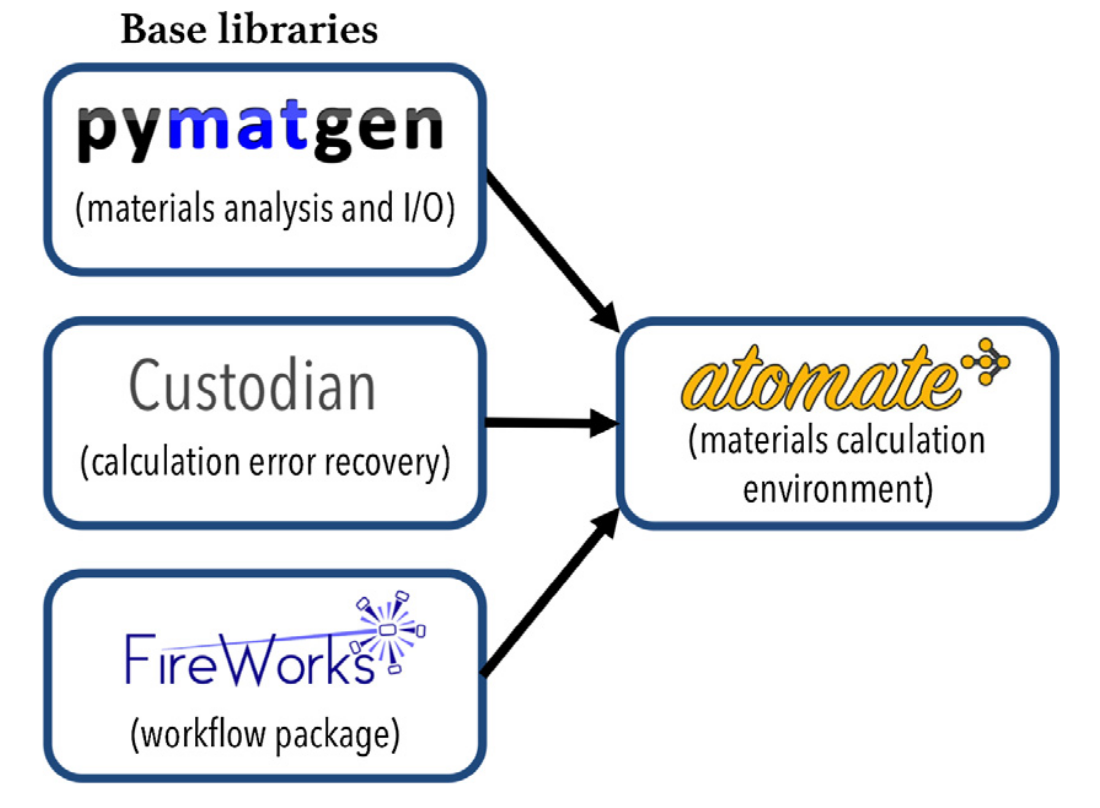
\includegraphics[height=1.4in,width=2.2in,viewport=0 0 820 630,clip]{Figures/Atomate_comp.png}
\vskip 1pt
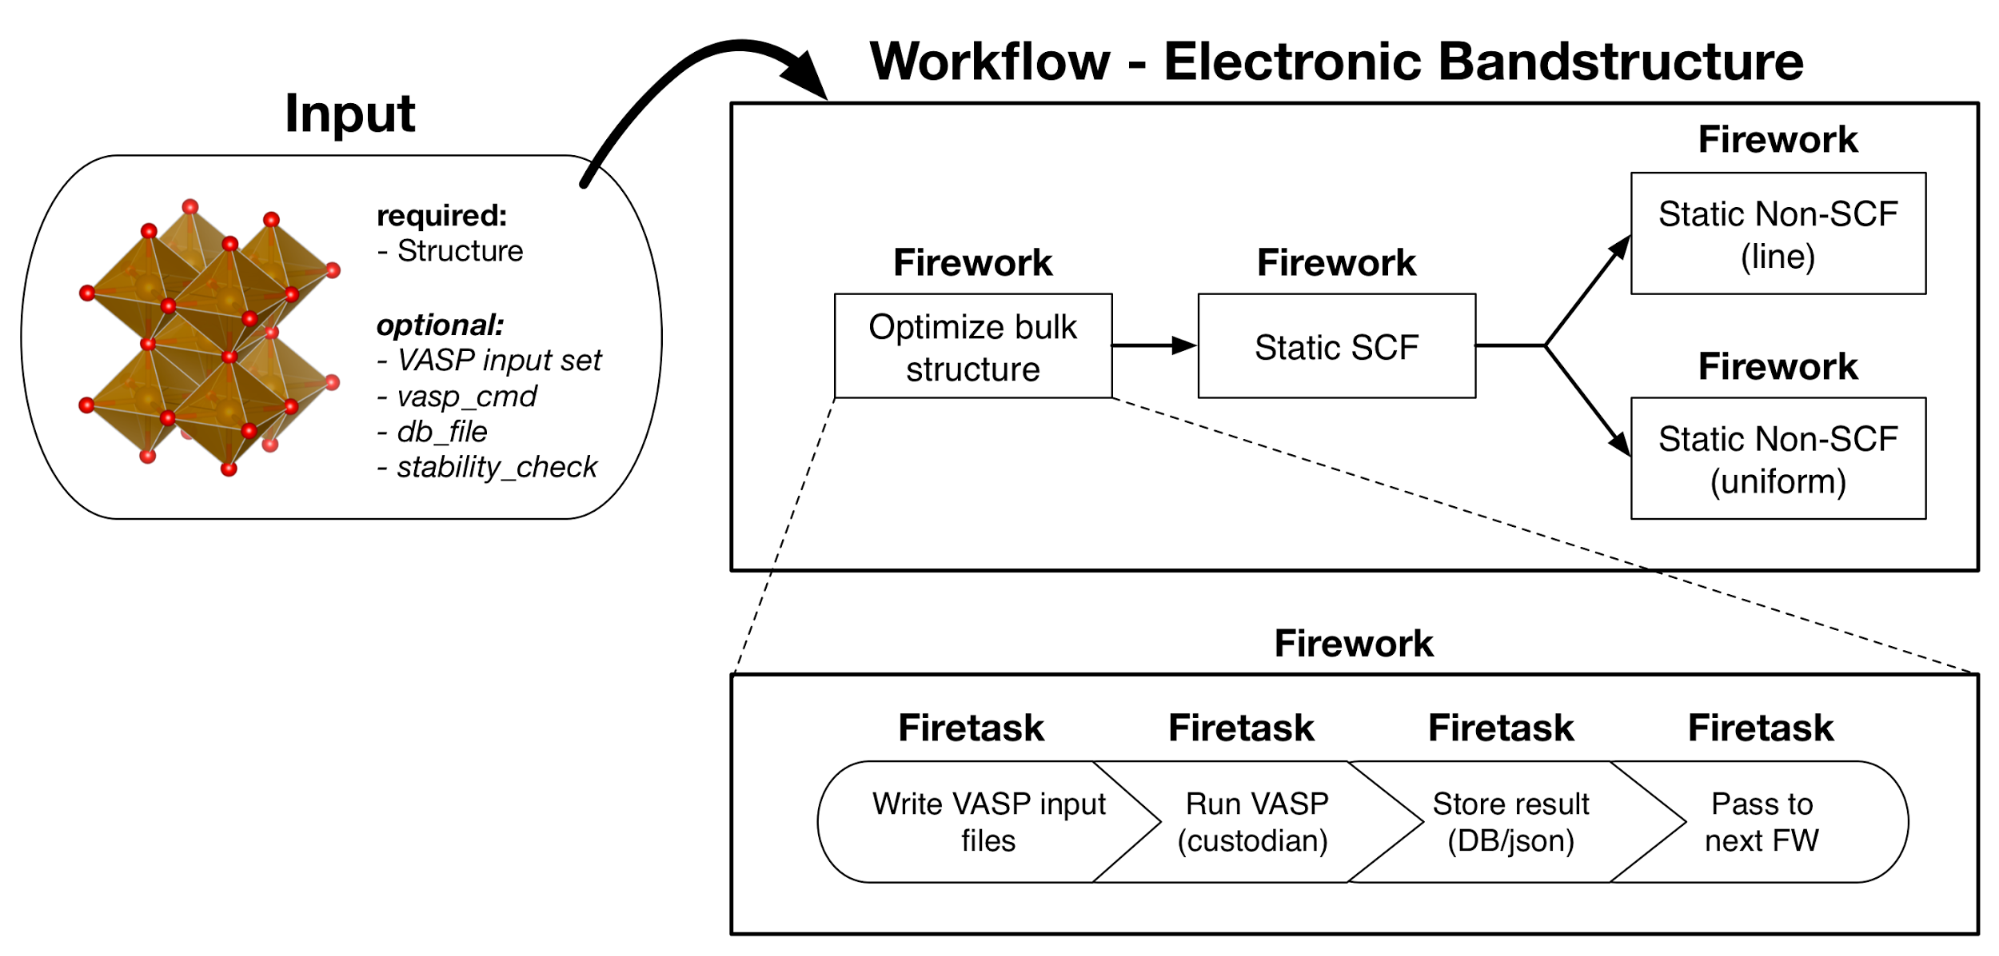
\includegraphics[height=1.5in]{Figures/bandstructure_wf.png}
%\caption{\fontsize{7.2pt}{4.2pt}\selectfont{\textrm{The integrated calculator in ASE (Atomic Simulation Environment).}}}%
\label{Logo_QM-MM}
\end{figure} 
}

\section{第一原理数据库}
\frame
{
	\frametitle{早期材料数据库:~\tt{SpingerMaterials}}
\textrm{SpingerMaterials}:~世界上最古老也是完备的材料数据库,旨在创建集成材料学信息、性质和使用平台
\vskip 3pt
数据库主要由以下部分组成:
\begin{itemize}
	\item 全部\textrm{Landolt-B{\"o}rnstein}丛书(自\textrm{1883}年起),是以基础科学为主的大型科学与技术数值与函数关系的工具书
	\item 全部\textrm{Pauling~File}无机材料数据库,收集了从\textrm{1900}年迄今超过\textrm{21000}种出版物中的无机晶体结构、衍射、相图和物理属性数据
	\item \textrm{Dortmud Data Band}中的纯液体和二元混合物的热物理数据
	\item 吸附材料数据库\textrm{(Adsorption Database)}
	\item 聚合物热力学数据库\textrm{(Polymer Thermodynamics Databse)}
	\item \textrm{MSI}数据库
\end{itemize}
}

\frame
{
	\frametitle{早期材料数据库:~其它数据库}
除\textrm{SpingerMaterials}之外,比较完整的数据有
{\fontsize{9.0pt}{4.2pt}\selectfont{
\begin{itemize}
	\item 无机晶体结构数据库\textrm{(Inorganic Crystal Structure Database, ICSD)}:~\url{http://www.fiz-karlsruhe.com/icsd.html}%\cite{ICSD_URL},
		\vskip 2pt
{\fontsize{6.5pt}{4.2pt}\selectfont{服务器位于德国的\textrm{FIZ~Karlsruhe},收录了自\textrm{1913}年以来超过\textrm{185000}条矿物、 金属和其他无机固体化合物(含\textrm{2000}多元素单质、\textrm{34500}多二元化合物、\textrm{68000}多三元化合物、\textrm{66000}多四元及多元化合物)的晶体结构数据}}
%类似的实验材料数据库还有
\item \textrm{CRYSTMET}数据库%:~\url{http://www.tothcannda.com/database.htm}%\cite{CRYSTMET_URL}、
\item \textrm{Pauling}无机材料数据库:~\url{http://www.paulingfile.com/}%\cite{Pauling_URL}
\item \textrm{Pearson}晶体数据库:~\url{http://www.crystalimpact.com/}%\cite{Pearson_URL}
\item $\cdots$
\end{itemize}}}
\textcolor{blue}{这些实验数据库对于材料学研究提供了重要的帮助}

%但是仅有这些数据库肯定是不够的,一方面
\begin{itemize}
	\item 材料的覆盖范围非常广泛,有限的数据库不可能穷尽%,更重要的是
	\item 有很多材料的物性数据很难通过实验直接得到
\end{itemize}

%材料设计和开发是复杂的多维优化问题,注定新材料研发耗时耗力%。在这一点上,
原子尺度的材料物性数值模拟可以有效补偿实验方法的不足\\
%近年来雨后春笋般的计算材料数据库填补了不少很多实验数据缺乏的空白%\cite{CMS58-227_2012},
\textcolor{red}{集成了实验数据和计算数据的新材料数据库为探索新材料合成、性能优化开辟了新的研究思路}

%随着高性能计算与\textrm{DFT}相结合推动了第一原理材料模拟数据生成和结果分析的自动化,%而随着“材料基因组计划”的实施,为计算材料科学提供了越来越广阔的应用空间,也
%涌现了越来越多的计算材料数据库,特别是在功能材料领域,高通量\textrm{DFT}计算大大推进了新材料研发的进步。%\cite{JCED59-3232_2014, IC53-11849_2014,JPCL4-3607_2013,PCCP16-22073_2014}
}

\frame
{
\frametitle{\tt{AFLOWLIB}}
%\subsubsection{\tt{AFLOWLIB}}
\textrm{AFLOWLIB}是由高通量\textrm{DFT}计算框架\textrm{AFLOW}%\cite{CMS58-218_2012,CMS58-227_2012,Nat-Mater12-191_2013}
生成的材料信息数据库:~\url{https://www.aflowlib.org}
\vskip 3pt
{\fontsize{7.5pt}{4.2pt}\selectfont{该数据库涵盖相图、电子结构和磁学性质等信息,源代码和主要材料数据由\textrm{Duke}大学开发和运维}}%\cite{AFLOWORG_URL},
\begin{itemize}
	\item 数据库包含\textrm{630,000}种以上的合金热力学条目,涵盖了\textrm{ICSD}中的\textrm{52,000}多种化合物,\textrm{3,000}多种基本化合物,\textrm{330,000}多种二元化合物和\textrm{262,000}多种\textrm{Heuslers}金属间化合物
	\item 数据库提供在线的界面搜索,包括计算的细节、电子结构、磁学性质和热力学性质,所有的计算结果都是由\textrm{AFLOW}高通量计算软件生成的
	\item 计算数据在数据库种以\textrm{SQL}(\textrm{MySQL})形式存储,检索方便
		\vskip 2pt
		{\fontsize{7.5pt}{4.2pt}\selectfont{\url{https://www.aflowlib.org}提供数据交换的应用接口\textrm{RESTful~API}服务}}%\cite{CMS93-178_2014},
\end{itemize}
数据库种的材料数据可以表示为多种格式,包括\texttt{HTML/JSON/DUMP/PHP/TEXT/NONE}等,极大地方便了用户在新材料研发中的数据挖掘需求
}

\frame
{
\frametitle{\tt{MP}}
%\subsubsection{\tt{MP}}
\textrm{Materials Project}是美国材料基因组项目项目支持高通量第一原理计算的软件和数据库:~\url{https://www.materialsproject.org}%\cite{MP_URL},
\vskip 2pt
{\fontsize{8.5pt}{4.2pt}\selectfont{\textrm{MP}基于\textrm{Apache}、\textrm{Python}和\textrm{Django}开发,在开源软件平台\textrm{github}上发布全部代码,面向全世界的开发者支持:~\url{https://gitbub.com/materialsproject}}}
\vskip 3pt
根据\textrm{MP}官网信息,目前可提供的数据包括:
\begin{itemize}
	\item \textrm{59,000}多种化合物的信息,\textrm{41,000}多种能带结构数据和\textrm{1,300}多种材料的弹性张量数据
	\item \textrm{2,200}多种\textrm{\ch{Li}}的插层电极和\textrm{19,000}多种\textrm{\ch{Li}}的转换电极数据
	\item \textrm{Materials Project}的扩展性极好\\
		{\fontsize{8.0pt}{4.2pt}\selectfont{除了\textrm{Pymatgen}、\textrm{FireWorks}和\textrm{Custodian}的支持,其数据库采用基于\textrm{MongoDB}的\textrm{NoSQL}数据格式文件,%因为传统的数据库只是“纵向可扩展”\footnote{\fontsize{5.0pt}{4.2pt}\selectfont{横向可扩展,是指数据库可支持增加数据库的服务器数目;~纵向可扩展是指数据库可支持增加硬盘、内存和\textrm{CPU}的数目}},\textrm{NoSQL}数据库
	弥补了传统数据库的扩展性差和灵活性不够的问题}}%,近年来在材料研究数据库技术中特别受到注意
\end{itemize}

\textrm{Materials Project}同样通过\textrm{API}支持\textrm{RESTful}服务%\cite{CMS68-314_2013},
%根据\textrm{RESTful}的设计,对数据的需求和操作,不须依赖复杂的用户界面,只要直接对数据库的\textrm{URL}完成。\textrm{RESTful}接受到\textrm{URL},\textrm{Materials Project}材料数据库返回的\textrm{JSON}结构。\textrm{RESTful}服务器有效地提升了数据获取效率,如\textrm{Pymatgen}的结构对象,\textrm{生成能}、\textrm{VASP}计算结果等。对科研工作者而言,\textrm{RESTful}是有效的研究工具。
}

\frame
{
\frametitle{\tt{CMR}}
%\subsubsection{\tt{CMR}}
\textrm{CMR}和\textrm{ASE}都是由丹麦技术大学\textrm{QMIP}项目开发的\\
{\fontsize{7.5pt}{4.2pt}\selectfont{\textrm{ASE}主要服务第一原理计算任务生成、计算执行、结果分析和可视化}}\\
\textrm{CMR}则主要面向计算数据存储:~\url{https://cmr.fysik.dtu.dk}
%{\fontsize{8.5pt}{4.2pt}\selectfont{当前\textrm{ASE}和\textrm{CMR}仍在开发中,不断发布更新的稳定版本}},有比较完整的安装、使用说明文档。
\begin{itemize}
	\item \textrm{CMR}提供了超过\textrm{30,000}条数据记录
	\item \textrm{CMR}提供了三种不同的用户界面\textrm{PHP/HTML和Python},方便不同经验的用户存储、检索电子结构计算数据%\cite{CMR_URL},\cite{CSE14-51_2012},
\end{itemize}
与\textrm{ASE}类似,\textrm{CMR}面向用户对数据库的多元化需求,实现软硬件的尽可能兼容
{\fontsize{7.5pt}{4.2pt}\selectfont{
\begin{itemize}
	\item 软件方面:~\textrm{ASE}和\textrm{CMR}所有源代码开发都是基于松耦合模式,方便用户根据习惯使用软件\\
		{\fontsize{6.0pt}{4.2pt}\selectfont{主要是面向开源系统,特别是\textrm{Linux}操作系统,\textrm{Apache}浏览器,\textrm{MySQL}数据库,用户界面采用\texttt{PHP/HTML},合成\textrm{LAMP}(\textrm{Linux,Apache,MySQL,PHP})套装}}
		%。比如用户可以分别只选用\textrm{ASE}或\textrm{CMR};
	\item 硬件方面,软件可以安装到台式机、集群或超级计算机上,对于小的台式机则无须安装数据库和网络服务器
	\item \textrm{CMR}使用\textrm{SQLite}数据库模式而不用\textrm{MySQL}服务器模式存储和检索材料数据\\
		{\fontsize{6.0pt}{4.2pt}\selectfont{当用户有需要时,\textrm{CMR}的数据处理模块可将\textrm{SQLite}数据库文件上传到\textrm{MySQL}服务器上,或者将数据文件转呈\texttt{XML/JSON}格式,以方便数据交换}}
\end{itemize}}}
}

\frame
{
\frametitle{\tt{ESP}}
%\subsubsection{\tt{ESP}}
\textrm{ESP}的数据库是\textrm{Uppsala}大学为加速新的功能材料的研发进程而开发的:~\url{http://gurka.fysik.uu.se/ESP/}
\begin{itemize}
	\item \textrm{ESP}数据库中的电子结构数据是依据\textrm{ICSD}的无机化合物的结构数据,由\textrm{FP-LMTO}方法通过第一原理计算产生\\
{\fontsize{6.5pt}{4.2pt}\selectfont{自2002年\textrm{ESP}发布以来,共收录了\textrm{60,000}多条化合物的电子结构数据}}
\item 用户最多允许查阅含有五种元素的化合物的电子结构信息
\end{itemize}
应用数据挖掘技术,由\textrm{ESP}的\textrm{60,000}多条化合物电子结构信息,已经预测了17种潜在可能的强拓扑绝缘体\\%\cite{arXiv1007-4838_2010,APR6-31_2014},
{\fontsize{7.5pt}{4.2pt}\selectfont{\textrm{ESP}的官网提供的信息显示:~采用大规模计算结合数据挖掘技术提供的17种可能的化合物中,成功预测到了第一个强拓扑绝缘体\textrm{(toplogical insulator)}\textrm{\ch{Bi2SeTe2}},而且预测很快就得到验证}}

\textrm{ESP}的数据库和能带分析工具的代码都没有公开\\
近年来,\textrm{ESP}数据库开发进展缓慢
}

\frame
{
\frametitle{\tt{ESTEST}}
%\subsubsection{\tt{ESTEST}}
\textrm{ESTEST}是加州大学\textrm{Davis}分校%\textrm{(the University of California at Davis)}
开发的材料数据库:\\\url{http://estest.ucdavis.edu/}\\%\cite{ESTEST_URL,CSD3-015004_2010,CPC183-1744_2010}
{\fontsize{6.5pt}{4.2pt}\selectfont{用于软件\textrm{Qbox}、\textrm{VASP}、\textrm{Quantum Espresso}、\textrm{Siesta}、\textrm{ABINI}的结果和电子结构计算软件\textrm{Exciting}的结果检验和对比}}

通过数据库的网页界面,可将各类软件的输入/输出文件转换成统一的\textrm{XML}格式,便于数据存储、比较、分析\\
{\fontsize{6.5pt}{4.2pt}\selectfont{每个\textrm{XML}文件由文件名和数据库存储位置区别}}
{\fontsize{7.5pt}{4.2pt}\selectfont{
\begin{itemize}
	\item \textrm{ESTEST}数据库总共包括\textrm{400}多条\textrm{Qbox}的计算记录,\textrm{10}条左右的\textrm{VASP}计算记录,\textrm{Quantum Espresso}和\textrm{Siesta}计算记录各\textrm{70}多条,\textrm{150}多条\textrm{ABINIT}计算记录,\textrm{Exciting}的记录约\textrm{30}条
	\item \textrm{ESTEST}的网页界面提供了类似\textrm{Google}的简明搜索栏,网页还提供了多个搜索下来菜单,可根据软件名称、计算元素等检索

	\item 数据库的网页界面可提供数据、表格和图片形式的电子结构的模拟信息:\\
		{\fontsize{6.5pt}{4.2pt}\selectfont{包括计算参数、原子信息、能量结果和结构应力与光谱信息}}

	\item 网页界面还提供了一些插件,可对诸如原子距离、晶格、能带结构、态密度、能量和结构应力或其他记录转换成一种或多种数据格式\\
{\fontsize{6.5pt}{4.2pt}\selectfont{例如\textrm{band\_structure\_plot}插件可将\textrm{XML}格式的能量本征值转成电子能带图}}\\
\end{itemize}
这种格式转换插件丰富了\textrm{ESTEST}生成、模拟计算结果的能力\\
需要说明的是:~必须是注册用户才能数据库的源代码}}
}

\frame
{
\frametitle{\tt{MAST}}
%\subsubsection{\tt{MAST}}
以完整的高通量框架的角度看,\textrm{MAST}更像是对\textrm{ESTEST}的辅助,重点用于工作流管理和后处理:\\
\url{http://pythonhosted.org/MAST/0_0_introduction.html}

\textrm{MAST}的基本框架由\textrm{MP}的\textrm{Pymatgen}和\textrm{Custodian}模块和\textrm{ASE}组合搭配实现
\vskip 2pt
{\fontsize{6.5pt}{4.2pt}\selectfont{\textrm{MAST}开发了自动计算流程以及数据库,而没有使用\textrm{FireWorks}和\textrm{MangoDB}}}
\vskip 2pt
\textrm{MAST}的数据主要来自\textrm{VASP}的数据拟合\\

\begin{itemize}
	\item \textrm{MAST}的数据库主要收集了带空位的稳定纯元素的数据,现有面心立方的\textrm{49}种元素和六方密堆积的\textrm{44}种元素
	\item \textrm{MAST}数据库主要用于研究基本的空位扩散,收集的数据包括:~空位形成焓、空位迁移焓、内聚能和体模量
\end{itemize}
\textrm{MAST}的数据生成和管理主要依赖于操作系统和\textrm{I/O}性能,运行\textrm{MAST}无须额外配置专门的数据库软件

\textrm{MAST}的数据目前还不能通过网页界面访问,很多功能还有待完善

}

\frame
{
\frametitle{\tt{CEPDB}}
%\subsubsection{\tt{CEPDB}}
\textrm{CEPDB}是哈佛大学的\textrm{CEP}项目的数据库:\\%\cite{CEPDB_URL,JPCL2-2241_2011}。
\url{https://gist.github.com/jessiegt/5642460f061a39d1820e}\\
主要服务于研究有机光电材料

根据\textrm{CEPDB}的网页信息显示,
\begin{itemize}
	\item 数据库共拥有\textrm{2,300,000}多个分子的图谱信息和\textrm{22,000,000}多个分子结构(由超过\textrm{150,000,000}个\textrm{DFT}计算得到)共计超过\textrm{400~TB}的数据,
	\item 数据库除了有第一原理计算结果,还收录了文献中的实验数据,用于作为\textrm{CEPDB}的训练和标定数据集
\end{itemize}
\textrm{CEPDB}使用\textrm{Python}的网页框架\textrm{Django}在\textit{in silico}上开发的高通量计算\textrm{MySQL}数据库,数据由量子化学计算软件\textrm{Q-Chem}得到\\
{\fontsize{6.5pt}{4.2pt}\selectfont{\textrm{CEPDB}的强大算力主要由\textrm{IBM}的公益分布式计算项目全球社群网格\textrm{(World Community Grid, WCG)}提供,还有一些算力来自\textrm{Harvard}的\textrm{FAS Odyssey}集群、\textrm{NERSC}和\textrm{TeraGrid}的计算资源以及其它一些计算资源}}

\textrm{CEPDB}的数据都是开放的,但高通量计算软件部分不开源\\不过\textrm{CEPDB}对全世界各研究组上传的实验数据持开放态度
}

\frame
{
\frametitle{\texttt{CCCBDB}}
%\subsubsection{\texttt{CCCBDB}}
计算化学对比和基准数据库\textrm{(Computational Chemistry Comparison and Benchmark Database, CCCBDB)}归属于美国国家标准和技术协会(\textrm{National Institute of Standards and Technology, NIST})

汇集了\textrm{1600}多种气相原子和分子的实验和第一原理计算的化学热力学数据,很好地弥补了常见数据库只有固体材料数据的不足

\begin{itemize}
	\item \textrm{CCCBDB}提供简单的在线服务界面,用户可以检索到指定化合物的实验数据和计算数据,实验和计算数据的对比也验证了数据的可靠性
	\item \textrm{CCCBDB}允许用户优先使用几何结构、振动模式、熵、能量和静电性质而非分子结构作为检索的关键词\\
		{\fontsize{7.5pt}{4.2pt}\selectfont{避免引入复杂的筛选组合,方便用户快速得到检索结果}}
	\item \textrm{CCCBDB}是一个庞大的数据库,收录了总计有超过\textrm{460,000}个计算条目\\
{\fontsize{7.5pt}{4.2pt}\selectfont{因为其没有开源,降低了数据库的影响力}}
\end{itemize}
}

\frame
{
\frametitle{\tt{AiiDA}}
%\subsubsection{\tt{AiiDA}}
\textrm{AiiDA}%\cite{AiiDA_URL}
是用于原子尺度材料自动模拟、管理、共享和复制的软件框架:~\url{http://www.aiida.net/}
\vskip3pt
{\fontsize{8.0pt}{4.2pt}\selectfont{软件由\textrm{THEOS-EPFL~(Theory and Simulation of Materials-{\'E}cole~Polytechnique~F{\'e}d{\'e}rale~de~Lausanne)}的实验室和\textrm{BOSCH}公司于2012年开发和维护}}
\vskip 3pt
\textrm{AiiDA}数据库
\begin{itemize}
	\item 网页编程框架用\textrm{Python}维护
	\item 数据库用\textrm{Django}开发\\%\cite{CMS187-110086_2021},
		{\fontsize{7.0pt}{4.2pt}\selectfont{可满足计算物理、化学和材料科学研究的多种不同需求}}
\end{itemize}
数据库提供\texttt{SQLite/MySQL}和\texttt{PostgreSQL}三种形式的数据
\vskip 3pt
{\fontsize{8.0pt}{4.2pt}\selectfont{推荐使用\textrm{PostgreSQL}}}
\vskip 5pt
当用户使用数据库的\textrm{RESTful~API}接口时,数据将以\texttt{JSON}格式呈现
}

\frame
{
\frametitle{\tt{Alloy Database}}
%\subsubsection{\tt{Alloy Database}}
\textrm{Alloy~Database}数据库
提供\textrm{VASP}计算的合金结构和结合能数据,%\cite{AlloyD_URL},
其在线服务器位于卡内基梅隆大学\textrm{(Carnegie~Mellon~University)}物理系:
\url{http://alloy.phys.cmu.edu}
\vskip 3pt
\textrm{Alloy~Database}数据库的主要功能
\begin{itemize}
    \setlength{\itemsep}{5pt}
	\item 包括\textrm{200}多种二元合金、\textrm{100}多种三元合金和\textrm{20}多种四元合金的材料数据
	\item 用户可以检索二元、三元和四元合金的\textrm{VASP}计算数据
	\item 数据库提供包括合金组分的元素信息、\textrm{Pearson}符号、合金模型以及计算所需的\textrm{POSCAR}文件、合金\textrm{Pearson}符号,基态总能和生成焓、化学组成和赝势等
\end{itemize}
\textrm{Alloy~Data}最早于\textrm{2006}年提供线上服务,由于其数据库服务代码从未开放,所以该数据库迄今尚未应用于高通量第一原理计算
}

\frame
{
\frametitle{\tt{NoMaD}}
%\subsubsection{\tt{NoMaD}}
{\fontsize{8.0pt}{4.2pt}\selectfont{
\textrm{Novel Materials Discovery~(NoMaD)}是面向第一原理计算的电子结构数据生成、组织和交换的重要材料数据库:~\url{http://nomad-repository.edu/cms/}%\cite{NoMaD_URL}。
\vskip 3pt
当前\textrm{NoMaD}数据库
\begin{itemize}
	\item 包含\textrm{640,000}多条数据\\
		{\fontsize{6.0pt}{4.2pt}\selectfont{其中有\textrm{250,000}多条数据来自\url{http://aflowlib.org},其余则来自\url{http://cccbdb.nist.gov}}}
	\item 通过网页~\url{http://nomad-repository.edu/gui/\#nomad}共享数据
	\item 用户可通过元素、结构和计算方法、作者等信息检索到目标数据
	\item 供下载的数据主要是计算所需的输入/输出文件的压缩包\\
{\fontsize{6.0pt}{4.2pt}\selectfont{少量关于计算本身(如材料的化学式、空间群、计算软件及版本、作者和参考文献等)}}
\end{itemize}
{\fontsize{7.0pt}{4.2pt}\selectfont{\textrm{NoMaD}目前可支持的计算软件数据涵盖:~\textrm{ABINIT}、\textrm{CASTEP}、\textrm{CRYSTAL}、\textrm{Exciting}、\textrm{FHI-aims}、\textrm{Gaussian}、\textrm{Quantum-Espresso}、\textrm{VASP}和\textrm{WIEN2k}等}}
\vskip 3pt
{\fontsize{7.5pt}{4.2pt}\selectfont{\textrm{NoMaD}的注册用户不仅可以浏览和下载材料数据,还允许向\textrm{NoMaD}上传数据
\vskip 2pt
	{\fontsize{6.0pt}{4.2pt}\selectfont{用户可指定上传文件为“开放”\textrm{(open access)}或“限制”\textrm{(restricted)}状态}}
%\begin{itemize}
%	\item “开放”态:~对全体互联网用户开放
%	\item “限制”态:~只对指定用户群开放。
%\end{itemize}
\vskip 3pt
\textrm{NoMaD}的绝大部分数据(约\textrm{540,000}多条)是开放的,而“限制”状态的数据最多三年后自动转成“开放”状态,确保科学材料数据最大限度的共享和交换能力
\vskip 3pt
\textrm{NoMaD}除了提供材料计算的输入/输出文件,未提供高通量计算框架,一些重要的和有价值的材料数据{\fontsize{6.0pt}{4.2pt}\selectfont{(如计算参数以及计算能量数据)}}在数据文件下载之前已被隐去}}
}}
}

\frame
{
\frametitle{{\tt OQMD}与\tt{qmpy}}
%\subsubsection{\tt{OQMD}与\tt{qmpy}}
{\fontsize{8.0pt}{4.2pt}\selectfont{
开放量子材料数据库\textrm{(Open Quantum Materials Database, OQMD)}是\textrm{2013}年前后,由美国西北大学\textrm{(Northwestern University)}的研究团队在超过\textrm{200,000}个\textrm{DFT}计算的晶体结构基础上发展起来的:~\url{http://oqmd.org/}
\vskip 2pt
{\fontsize{6.0pt}{4.2pt}\selectfont{数据主要是在西北大学高性能计算队列和美国国家能源研究科学计算中心\textrm{(the National Energy Research Scientific Computing Center, NERSC)}的机器上完成}}

\begin{itemize}
	\item \textrm{OQMD}累积的\textrm{DFT}计算化合物约有\textrm{290,000}条
\vskip 2pt
{\fontsize{6.0pt}{4.2pt}\selectfont{这些化合物中约\textrm{10\%}来自\textrm{ICSD},约\textrm{90\%}来自简单化合物雏形组合,数据库中的化合物条目仍在增加}}
	\item 数据库收录的\textrm{DFT}计算的材料热力学和结构性质数据可以在线共享%\cite{OQMD_URL,NCM1-15010_2015},
	\item 数据库没有提供\textrm{RESTful}服务,但允许用户在\textrm{URL}地址栏输入检索化合物的字符串
		\vskip 2pt
		{\fontsize{6.0pt}{4.2pt}\selectfont{如~\textrm{\url{http://oqmd.org/materials/composition/Al2O3}}~表示\textrm{\ch{Al2O3}}的检索}}
\end{itemize}
{\fontsize{7.0pt}{4.2pt}\selectfont{软件\textrm{qmpy}是\textrm{OQMD}的\textrm{Python}的\textrm{API}:~\url{http://oqmd.org/static/docs/index.html}%\cite{qmpy_URL}
%和全部近\textrm{300,000}个结构数据可下载
\vskip 3pt
\textrm{qmpy}用\textrm{Django}开发,数据库是\textrm{MySQL}形式,数据主要由\textrm{VASP}计算得到}}
\vskip 5pt
通过浏览器得到的\textrm{OQMD}检索数据是\texttt{HTML}格式的(而非\texttt{JSON}或\texttt{XML}格式的)
\vskip 3pt
\textrm{OQMD}允许用户将全部数据(约4\textrm{GB})下载到本地并保存成一个文件,对于小型的计算用户,这将提升用户对计算数据的掌控和分析能力}}
}

\frame
{
\frametitle{\tt{PyChemia}}
%\subsubsection{\tt{PyChemia}}
{\fontsize{8.0pt}{4.2pt}\selectfont{\textrm{Python Materials Discovery Framework~(PyChemia)}是近年来才出现的面向\textrm{DFT}的高通量计算框架
\begin{figure}[h!]
\centering
\vspace*{-0.15in}
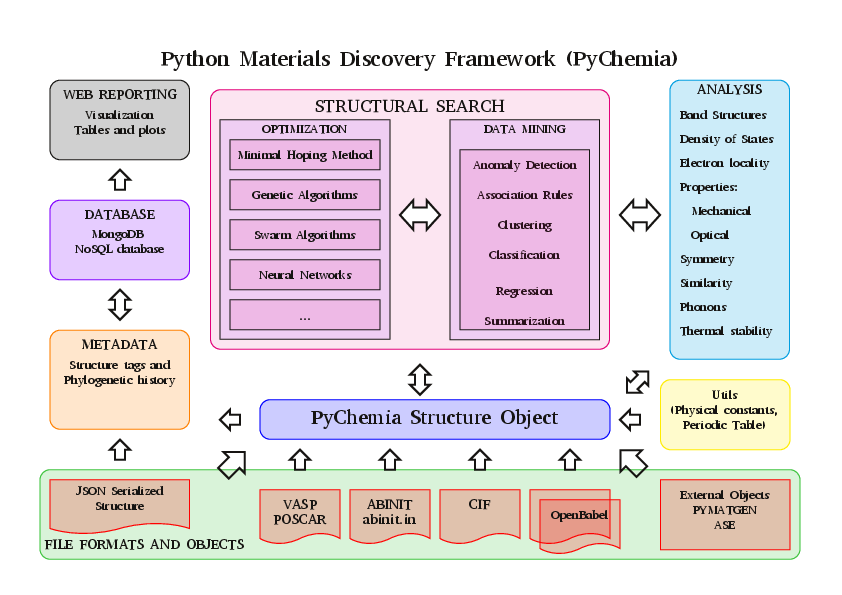
\includegraphics[height=2.3in]{PyChemia_code.png}
%\caption{\fontsize{7.2pt}{4.2pt}\selectfont{\textrm{The Framework of PyChemia.}}}%
\label{PyChemia_FireWork}
\end{figure} 
\textcolor{red}{目标}:~通过涵盖\textrm{DFT}计算和\textrm{Minima Hoping}等各种方法来推动发现新材料,并将\textrm{PyChemia}计算的数据存入数据库,作为后续发现新材料的备选化合物}}
}

\frame
{
\frametitle{\tt{PyChemia}}
{\fontsize{8.0pt}{4.2pt}\selectfont{\textrm{PyChemia}作为\textrm{Python}的一个模块,全部代码是最初于\textrm{2014}年由西弗吉尼亚大学\textrm{(West Virginia University)}分享到\textrm{GitHub}网站:\\
\url{http://github.com/MaterialsDiscovery/PyChemia}%\cite{PyChemia_Github},

\textrm{PyChemia}的新特色
\begin{itemize}
	\item \textrm{PyChemia}可支持的\textrm{DFT}计算软件涵盖\textrm{VASP}、\textrm{ABINIT}、\textrm{Octopus}、\textrm{DFTB+}和\textrm{Fireball}等
	\item 利用\textrm{Python}模块的特点,\textrm{PyChemia}完成了对\textrm{Pymatgen}、\textrm{ASE}和\textrm{qmpy}的集成
	\item 相比于其他高通量材料计算软件,\textrm{PyChemia}更显著的特长是材料结构搜索,而不是简单的材料计算和数据采集
		\vskip 2pt
		{\fontsize{6.0pt}{4.2pt}\selectfont{\textrm{PyChemia}除了提供大的材料数据库作为结构搜索的基础,还可以将每一套结构搜索产生新的小型数据库}}
\end{itemize}
\vskip 3pt
%图\ref{PyChemia_FireWork}给出了\textrm{PyChemia}的代码框架。
\textrm{PyChemia}采用\textrm{MongoDB}的\textrm{NoSQL}数据库而非传统的关系型数据库形式,方便产生结构搜索需要的小型数据库
\vskip 2pt
{\fontsize{6.0pt}{4.2pt}\selectfont{为兼顾不同\textrm{DFT}计算软件包材料结构以及各种物理性质研究的需要}}
\vskip 3pt
\textrm{PyChemia}由\textrm{Python}、\textrm{Django}和\textrm{MongoDB}搭建而成,其中\textrm{Django}是\textrm{PyChemia}用于显示计算的网页前端

目前\textrm{PyChemia}仍在开发中,尚未发布稳定版本的软件}}
}

\frame
{
	\frametitle{\tt{Atomly}}
\textrm{Atomly}材料科学数据库%\cite{ATOMLY_URL}
是中国科学院物理研究所刘淼研究员、孟胜研究员开发的第一原理材料数据库:~\url{https://www.atomly.net/}
\begin{figure}[h!]
\centering
\vspace*{-0.1in}
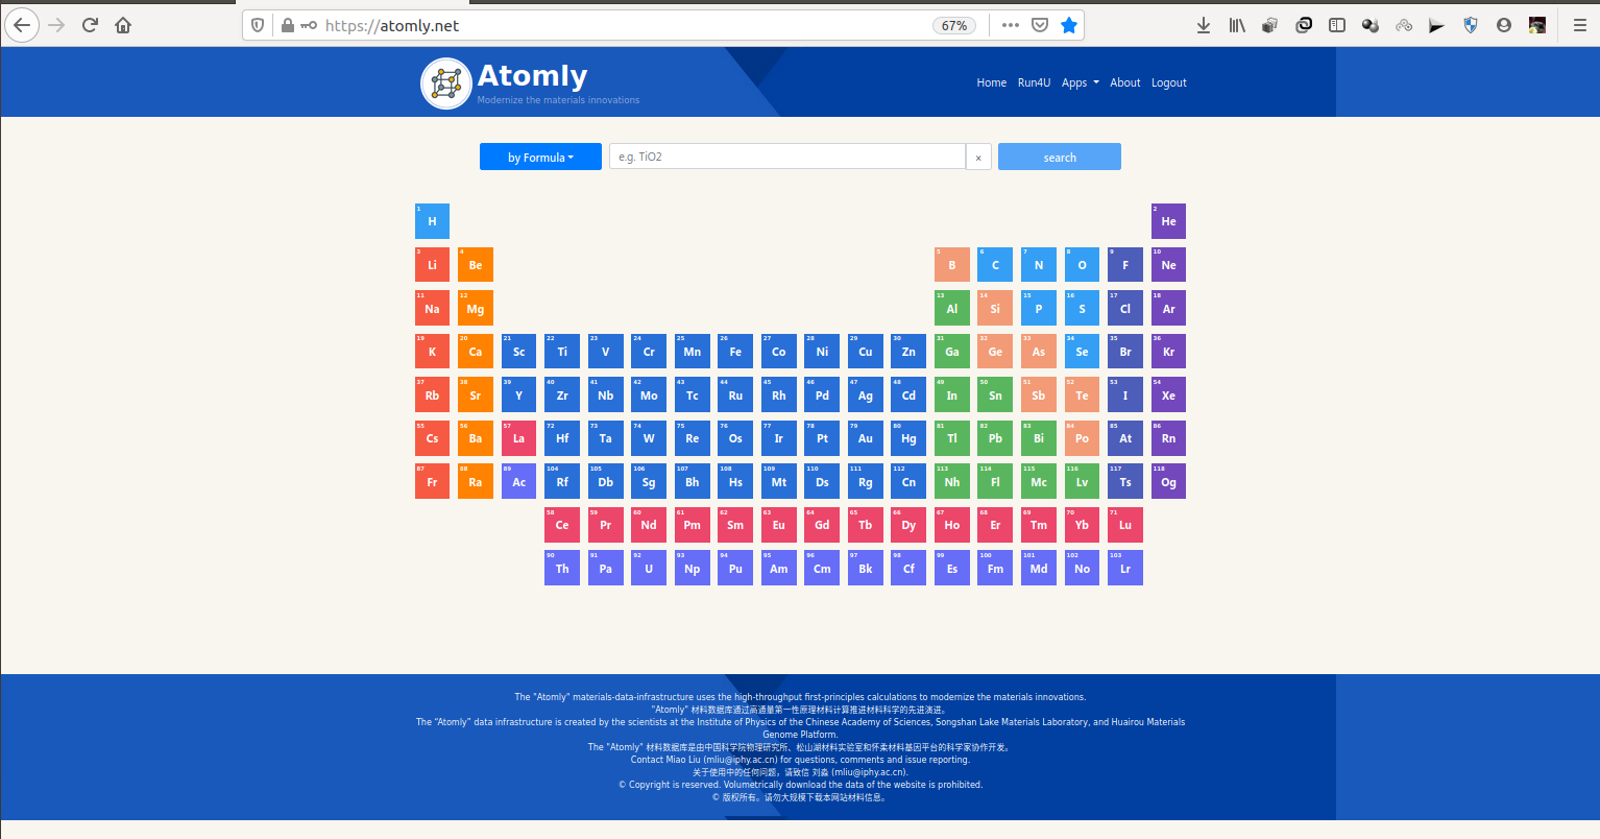
\includegraphics[height=2.1in,width=4.1in,viewport=5 0 1608 830,clip]{Figures/Atomly.png}
%\caption{\fontsize{7.2pt}{4.2pt}\selectfont{\textrm{Atomly:~中科院物理所~刘淼等老师开发,数据库包含了17万\!$^+$\!无机晶体材料第一性原理计算结果\textrm{(包含电子结构信息:~DOS~+~energy~bands)}.}}}%
\label{Logo_Atomly_lib}
\end{figure} 
}

\frame
{
\frametitle{\tt{Atomly}}
%\subsubsection{\tt{Atomly}}
%截止到目前已经收录了超过180,000条无机材料的高质量数据。
\textrm{Atomly}的\textcolor{red}{目标}:~为科研领域带来材料数据工具平台,通过数据驱动新材料的筛选、预测和发现,提升材料研发的生产力
\vskip 5pt
\textcolor{purple}{\textrm{Atomly}已收录\textrm{349,000+}种化合物,\textrm{342,00+}种能带结构和\textrm{68,000+}种相图数据}
\vskip 3pt
\begin{itemize}
	\item \textrm{Atomly}提供了性能优异的高通量第一原理计算流程框架\\
		{\fontsize{6.5pt}{4.2pt}\selectfont{依托中科院物理所的松山湖材料实验室的计算资源,框架支持的高通量计算流程可以支持~$10^3$数量级的材料体系同时计算}}
	\item \textrm{Atomly}的网页前端,提供便捷搜索,能快速定位到指定材料数据,并以友好的方式呈现给用户
	\item \textrm{Atomly}初步实践数据驱动的材料设计理念,能快速地完成高通量筛选,发现性能最优的候选材料
\end{itemize}
\vskip 5pt
借助人工智能算法,\textrm{Atomly}支持材料性质预测,能够以更快捷、更精准的范式预测材料结构和性质
}
%------------------------------------------------------------------------Reference----------------------------------------------------------------------------------------------
		\frame[allowframebreaks]
{
\begin{thebibliography}{99}
\frametitle{主要参考文献}
{\tiny
	\bibitem{CMS146-319_2018}\textrm{X. Yang, Z. Wang, X. Zhao and H. Liu \textit{Comp. Mater. Sci.}, \textbf{146} (2018), 319}
	\bibitem{url_Matcloud}\textrm{\url{http://matcloud.cnic.cn}}
	\bibitem{CMS58-227_2012}\textrm{S. Curtarolo, W. Setyawan, S. Wang, J. Xue, K. Yang, R. H. Taylor, L. J. Nelson, G. L. Hart, S. Sanvito, M. Buongiorno-Nardelli, N. Mingo and O. Levy \textit{Comp. Mater. Sci.}, \textbf{58} (2012), 227}
	\bibitem{CMS97-209_2015}\textrm{S. P. Ong, S. Cholia, A. Jain, M. Brafman, D. Gunter, G. Ceder and K. A. Persson. \textit{Comp. Mater. Sci.}, \textbf{97} (2015), 209}
	\bibitem{url_QMIP}\textrm{\url{http://www.qmip.org/qmip.org/Welcome.html}}
	\bibitem{JPCL2-2241_2011}\textrm{J. Hachmann, R. Olivares-Amaya, S. Atahan-Evrenk, C. Amador-Bedolla, R. S. S$\acute{a}$nchez-Carrera, A. Gold-Parker, L. Vogt, A. M. Brockway and A. Aspuru-Guzik \textit{J. Phys. Chem. Lett.}, \textbf{2} (2011), 2241}
	\bibitem{MPC4-148_2015}\textrm{L. Lin \textit{Mater. Perform. Character.}, \textbf{4} (2015), 148}
}
\end{thebibliography}
%\nocite*{}
}
